\documentclass[journal,10pt]{IEEEtran}
\pdfminorversion=7
\usepackage[T1]{fontenc}
\usepackage{newtxtext,newtxmath}
\usepackage{graphicx,booktabs,amsmath,array,multirow,xcolor}
\usepackage[hidelinks]{hyperref}
\usepackage{microtype}
\renewcommand{\topfraction}{0.92}
\renewcommand{\dbltopfraction}{0.92}
\renewcommand{\textfraction}{0.06}
\renewcommand{\floatpagefraction}{0.8}
\renewcommand{\dblfloatpagefraction}{0.8}
\newcommand{\RNE}{\operatorname{RNE}}
\title{Vela: An Efficient Open-Source FPGA Hardware Accelerator for End to End Vision-Language-Action Inference  }
\author{Cheng~Nian,~\IEEEmembership{Member,~IEEE,}
Jiaqi~Zhang, Fasih~Ud~Din~Farrukh, Jiaying~Peng, Xiaorui~Mo,\\
Fei~Chen,
Chun~Zhang,~\IEEEmembership{Senior Member,~IEEE}
\thanks{This work was supported in part by the Development and Reform Commission of Shenzhen Municipality under Grant XMHT20220115007. (Corresponding author: Chun Zhang.)}
\thanks{Cheng Nian and Fei Chen are with the Greater Bay Area National Center of Technology Innovation, Research Institute of Tsinghua University in Shenzhen, Shenzhen 518057, China (e-mail: \href{mailto:nc23@mails.tsinghua.edu.cn}{nc23@mails.tsinghua.edu.cn}).}
\thanks{Jiaqi Zhang, Fasih Ud Din Farrukh, Jiaying Peng, Xiaorui Mo, and Chun Zhang are with the School of Integrated Circuits, Tsinghua University, Beijing 100084, China (e-mail: \href{mailto:zhangchun@tsinghua.edu.cn}{zhangchun@tsinghua.edu.cn}).}}
\date{}
\begin{document}
\maketitle
\begin{abstract}
Low-bit arithmetic reduces the cost of vision--language--action (VLA) inference through compact data representation and dense matrix computation. Quantization groups also affect closed-loop task quality, while independently scaled partial sums and nonlinear operators require dedicated processing. This paper develops Vela, a W8A8 FPGA architecture with 64-element reduction groups. The design combines group-wise activation quantization and scale-aligned merging, DSP-pre-adder packing for two shared-activation products, and a heterogeneous nonlinear unit with shared elementwise and reduction paths. In 160 LIBERO episodes across eight tasks, the W8A8 G64 numerical implementation succeeds in 153 episodes, matching the floating-point total. Cycle-level evaluation gives 427.68 ms per policy invocation at 300 MHz, a 27.4\% latency reduction relative to the same-resource FP16 reference. The 768-DSP matrix array provides a theoretical peak of 921.6 GOPS. Post-route module results quantify the resource and power costs of quantization, merging, packed arithmetic, and nonlinear execution.
The architecture simulator and reproduction package are available at \url{https://github.com/nc-thu/vela}.
\end{abstract}
\noindent\textbf{Keywords:} vision--language--action, FPGA, group quantization, DSP packing, nonlinear acceleration.

\section{Introduction}\label{sec:intro}
Vision--language--action policies translate observations and instructions into robot actions. RT-2 transfers web-scale vision--language knowledge to robotic control~\cite{zitkovich2023rt2}, OpenVLA provides an open generalist manipulation model~\cite{kim2024openvla}, and $\pi_0$ couples pretrained vision--language representations to flow-based action generation~\cite{black2025pi0}. Their execution combines visual processing, interaction between modalities, and action prediction. TurboVLA reduces the dependence on a large language model by encoding vision and language separately and exchanging information through lightweight interaction modules~\cite{turbovla}. % ref:turbovla; anchor:abstract
The resulting workload still contains matrix operations, numerical conversions, nonlinear functions, and reductions. An FPGA implementation must support this mixture rather than optimize only an isolated dense layer.

Low-bit computation offers two immediate opportunities. Fewer weight bits reduce the amount of parameter data to move, and multiple narrow products can share a wider DSP multiplier. However, the number of bits also determines how accurately the policy represents its inputs and intermediate values. In a closed-loop robot task, numerical changes can alter later observations and decisions. The relevant design objective is therefore to reduce execution cost while preserving useful task performance, not simply to maximize products per DSP.

Three observations guide this work. First, quantization granularity strongly affects quality. In the evaluated selection set, changing W4A8 from a 64-element reduction group to a 32-element group increases success from 111/160 to 144/160. Smaller groups introduce more independently scaled partial sums, which the hardware must process. The same parameter that improves numerical resolution also changes the volume and frequency of merge work.

Second, packed multiplication requires support from the surrounding datapath. Pack2 produces two W8A8 products per DSP cycle, but the array must also recover signed fields, accumulate each group, and transfer its results for scale-aligned merging. In the W8A8 G64 model, matrix products account for 31.9\% of critical-path cycles, while data movement and layout account for 33.2\%. These costs motivate attention to operand delivery and the interfaces between packed arithmetic, group-result storage, and merging.

Third, nonlinear work remains substantial after matrix acceleration. In the W8A8 execution schedule, the nonlinear category accounts for 20.14\% of critical-path cycles. Elementwise activations and reduction-dependent functions also have different execution requirements. Normalization introduces serial dependencies, while exponentials and reciprocal operations consume separate arithmetic resources.

Existing approaches address parts of this problem. SmoothQuant redistributes quantization difficulty through an equivalent channel-wise transformation~\cite{smoothquant}. % ref:smoothquant; anchor:abstract
AWQ uses activation information to guide low-bit weight quantization~\cite{awq}. % ref:awq; anchor:abstract
DSP packing increases the arithmetic density of FPGA multipliers, with explicit attention to errors and corrections~\cite{dsppacking}. % ref:dsppacking; anchor:abstract
These mechanisms motivate useful arithmetic choices, but a grouped VLA datapath must additionally coordinate scale handling, partial-sum production, and heterogeneous operators.

The proposed architecture organizes these requirements into three hardware components. H1 provides the grouped quantization framework: it quantizes activations in reduction groups, buffers group results, and merges them using aligned scale coefficients. Its system evaluation compares the complete quantized architecture with a matched-resource FP16 array model. H2 maps two shared-activation INT8 products to each DSP pre-adder and multiplier using Pack2. H3 is a heterogeneous nonlinear unit (HNU) that combines piecewise-linear elementwise evaluation with reduction and special-function paths. Static-weight products and dynamic attention both use eight-bit operands.

The contributions are a workload-driven analysis of quantization granularity, an explicit W8A8 arithmetic mapping from grouped values to packed products and scale-aligned outputs, and an FPGA architecture study supported by closed-loop numerical evaluation, cycle modeling, and module implementation. The quality comparison motivates W8A8 G64 as the hardware configuration. The complete design reduces modeled invocation latency by 27.4\% relative to the matched-resource FP16 array reference. Mechanism comparisons separately examine the snapshot/merge organization, Pack2 density, and shared HNU datapath.

\begin{figure}[t]\centering
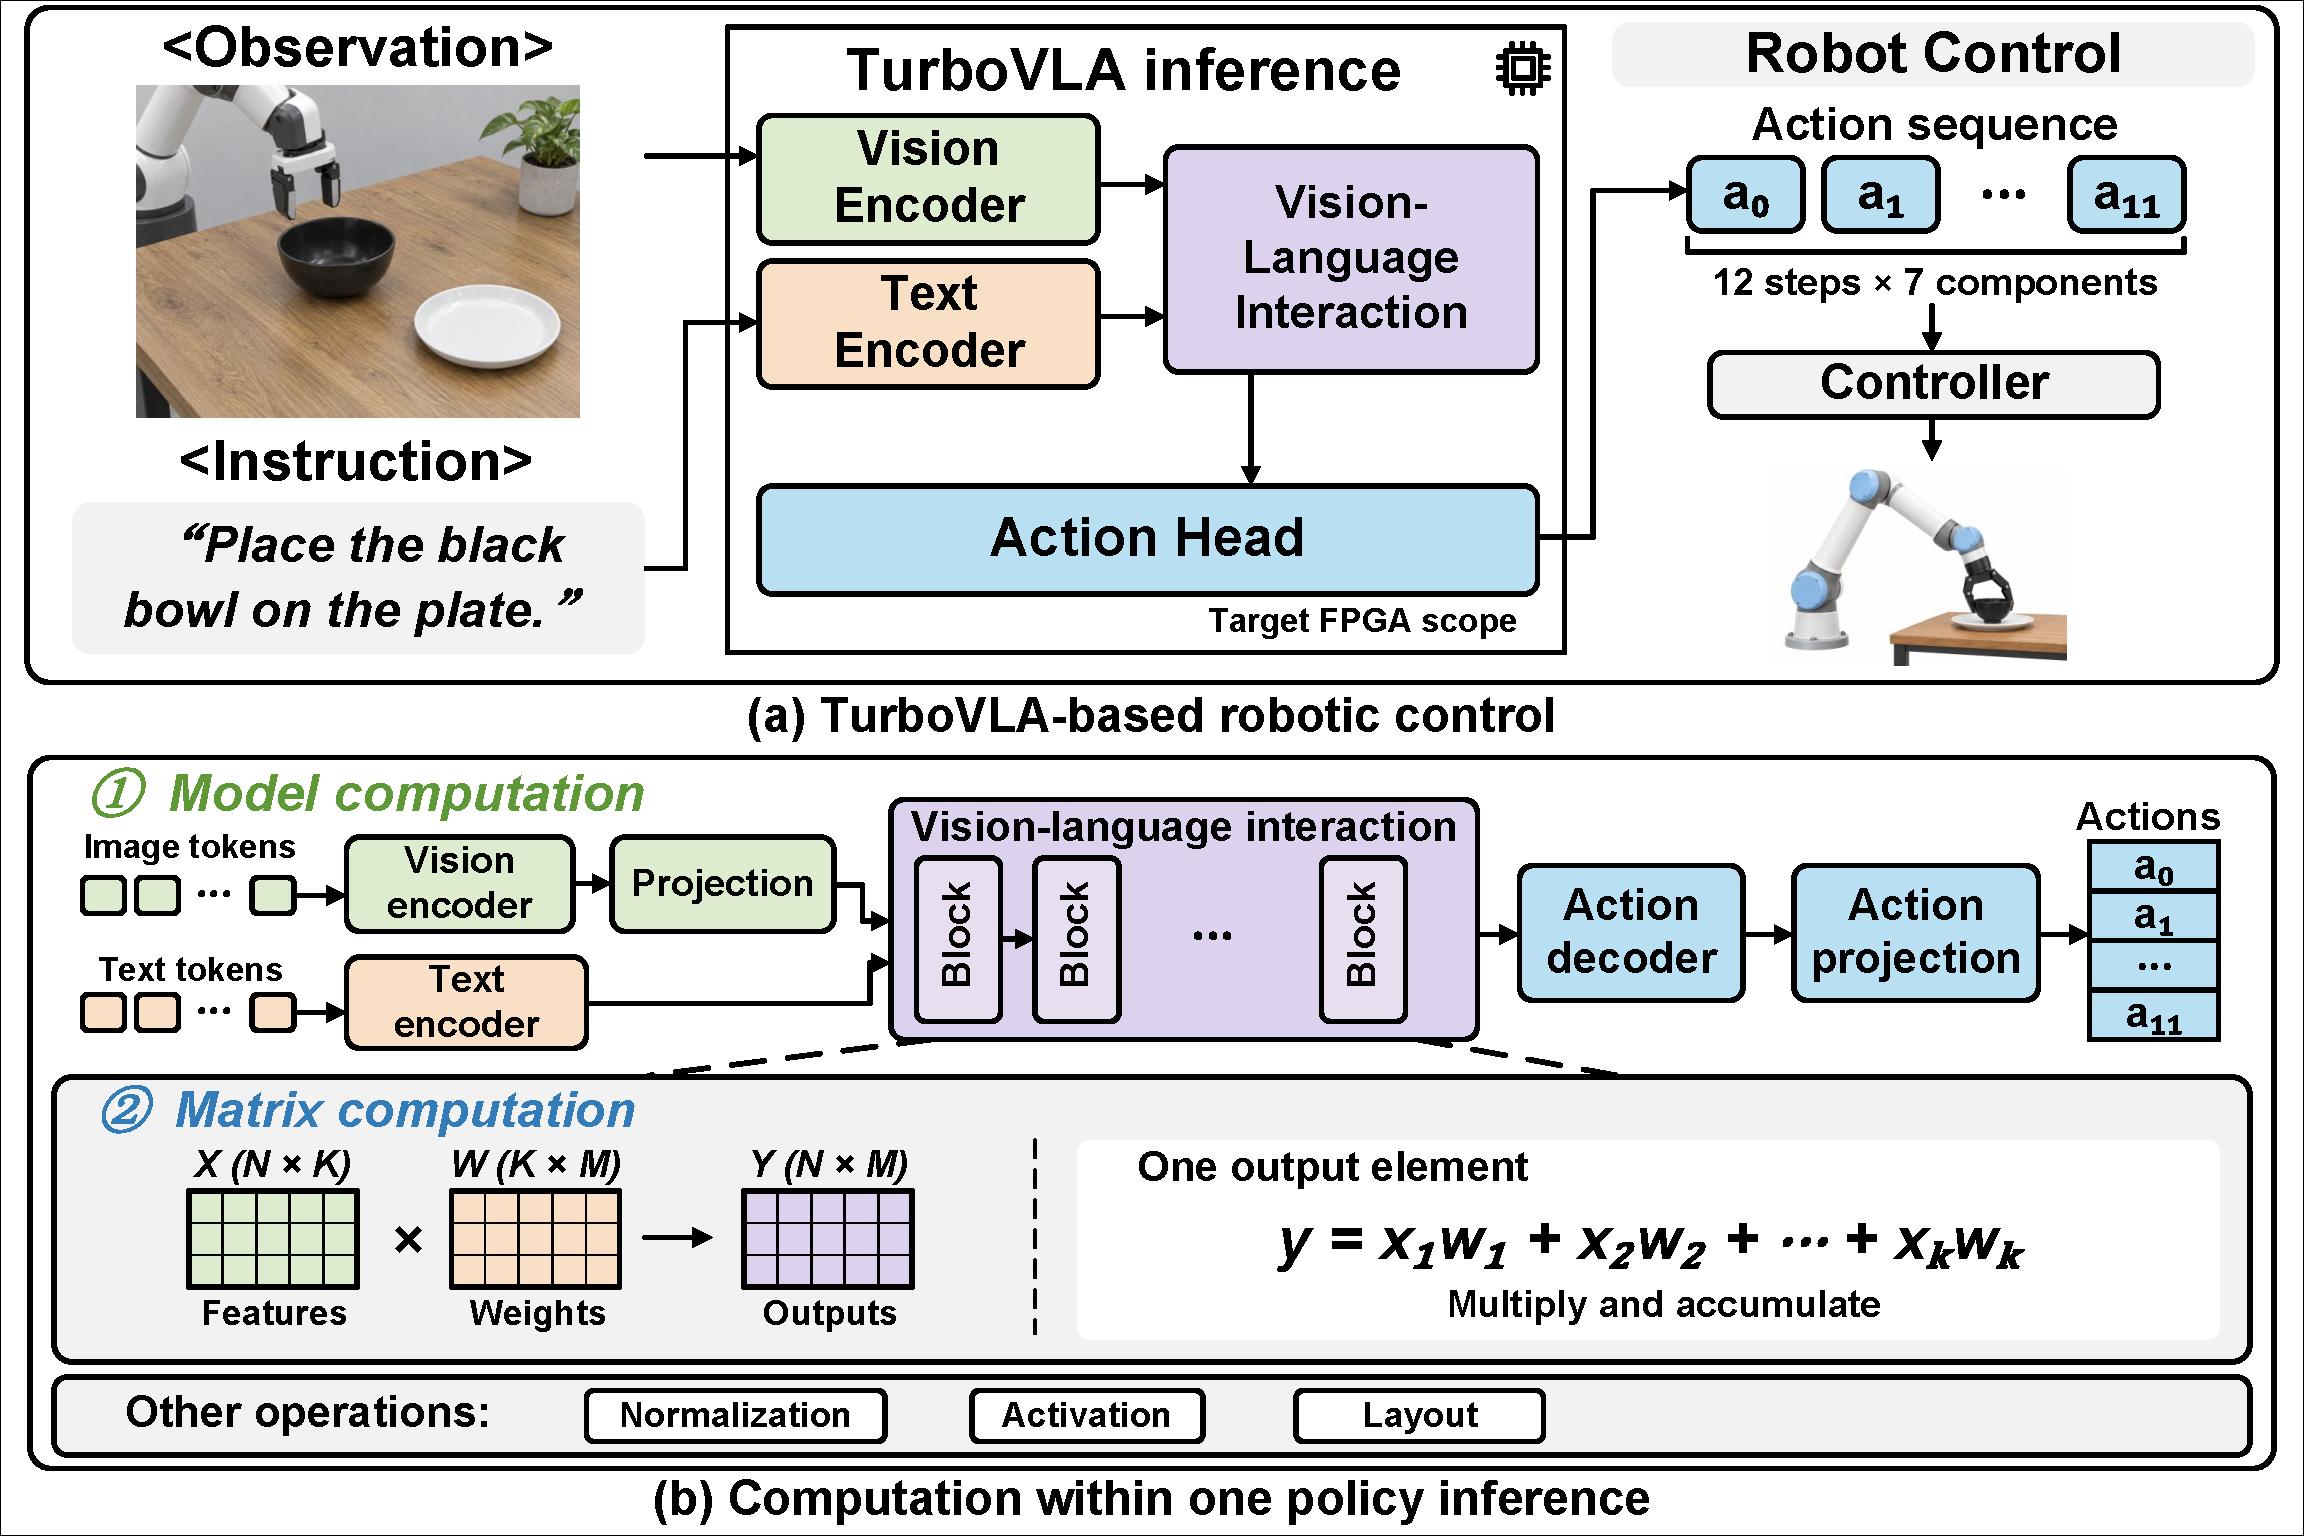
\includegraphics[width=\columnwidth]{figures/model.pdf}
\caption{TurboVLA workload. A policy invocation maps observations and instructions to a chunk of 12 seven-dimensional actions.}\label{fig:model}
\end{figure}

\section{Workload and Design Challenges}\label{sec:observations}
\subsection{VLA model organization}
VLA models differ in how semantic representations drive robot actions. CogACT conditions a specialized diffusion action transformer on vision--language features~\cite{li2024cogact}, while DiTA scales a diffusion-transformer policy for generalist control~\cite{hou2025dita}. SpatialVLA introduces 3D position information and adaptive spatial action grids~\cite{qu2025spatialvla}. SmolVLA emphasizes a compact model and decouples action prediction from execution through an asynchronous inference stack~\cite{shukor2025smolvla}. These designs make model organization and action execution part of the deployment problem. Vela studies the operator mixture of TurboVLA and selects arithmetic granularity using closed-loop task quality.

\subsection{Execution scope and precision notation}
Figure~\ref{fig:model} places the arithmetic in the policy workflow. The architecture trace contains 2,277 operators and 52,673,989,632 multiply--accumulate operations (MACs) per W8A8 G64 invocation. An invocation produces a chunk of 12 seven-dimensional actions. The execution policy consumes these actions and determines when to request the next invocation.

W8A8 denotes eight-bit static weights and eight-bit activations. The quality experiments also evaluate W4A8, which uses four-bit static weights and eight-bit activations. In attention products with two dynamic operands, both inputs remain eight-bit. The notation G64 or G32 specifies how many elements along the matrix reduction dimension $K$ share a scale. The hardware configuration uses W8A8 G64.

For an operation $Y=AB$, partitioning $K$ into $G$-element groups produces independently quantized subproducts. Activations require runtime statistics. Constant weights can be prepared offline, whereas a dynamic second operand needs runtime preparation. Both paths supply INT8 operands to the Pack2 datapath, while their scale metadata is prepared at different times.

\subsection{C1: Quality-sensitive grouping creates merge work}
The nine-configuration quality study compares the same eight tasks and 20 initial states per task. Its Direct baseline uses a tensor-wide activation scale and output-channel static-weight scales, without $K$ grouping. W8 Direct succeeds in 57/160 episodes, while W8 G64 succeeds in 153/160. W4 Direct succeeds in one episode. W4 G32 succeeds in 144. These differences establish that the representation granularity is consequential for this policy and selection set.

The useful group size also depends on precision. W4 G64 and G128 succeed in 111 and 105 episodes, respectively, below W4 G32. W8 G32 reaches 151 successes, compared with 153 for G64 and 152 for G128. These results motivate G64 for the W8 hardware configuration and demonstrate greater grouping sensitivity at four-bit weight precision.

Grouping also changes hardware demand. Each output element receives approximately $K/G$ partial sums, and each partial sum carries its own product of operand scales. Halving $G$ approximately doubles the number of group boundaries for a fixed, divisible $K$. The partial sums cannot be added as unscaled integers when those scales differ. Hardware must align them, accumulate them, and preserve sufficient numerical range.

An earlier schedule with a narrower merge organization illustrates the cost of group-result handling: changing W8 from G64 to G32 increases its critical-path merge contribution from 656,798 to 64,571,430 cycles. This observation motivates separating matrix production from group-result consumption and increasing the merge service rate.

\subsection{C2: Packed products require system support}
For shared activations, Pack2 generates two W8A8 products per DSP cycle. Sustaining this density requires input delivery, signed-field recovery, accumulator state, and downstream processing of completed groups.

The 48 physical columns expose 96 logical output columns under Pack2. At each group boundary, completed partial sums must be retained until their scale coefficients and merge lanes are available. If the merge or storage path cannot accept the results, the matrix array waits. The hardware must therefore coordinate packed multiplication with result storage and merge service.

In the W8A8 G64 invocation, matrix products occupy 40,873,040 critical-path cycles out of 128,304,013. Data movement and layout occupy another 42,626,787 cycles. These costs motivate coordinating packed arithmetic with operand delivery, snapshot storage, and group merging.

\subsection{C3: Nonlinear and reduction work remains visible}
The W8A8 G64 configuration assigns 25,833,842 critical-path cycles to the nonlinear category, corresponding to 86.11 ms at 300 MHz. The workload includes 20,366,568 Softmax input values, 23,722,512 LayerNorm input values, and 21,066,240 GELU input values per invocation.

GELU-like elementwise functions can be evaluated through independent coefficient lookups and multiply-adds. Softmax needs a row reduction, exponentials, another reduction, and normalization. LayerNorm similarly depends on statistics shared across a row. These dependencies motivate H3's division into elementwise, reduction, and special-function resources.

\begin{figure*}[t]\centering
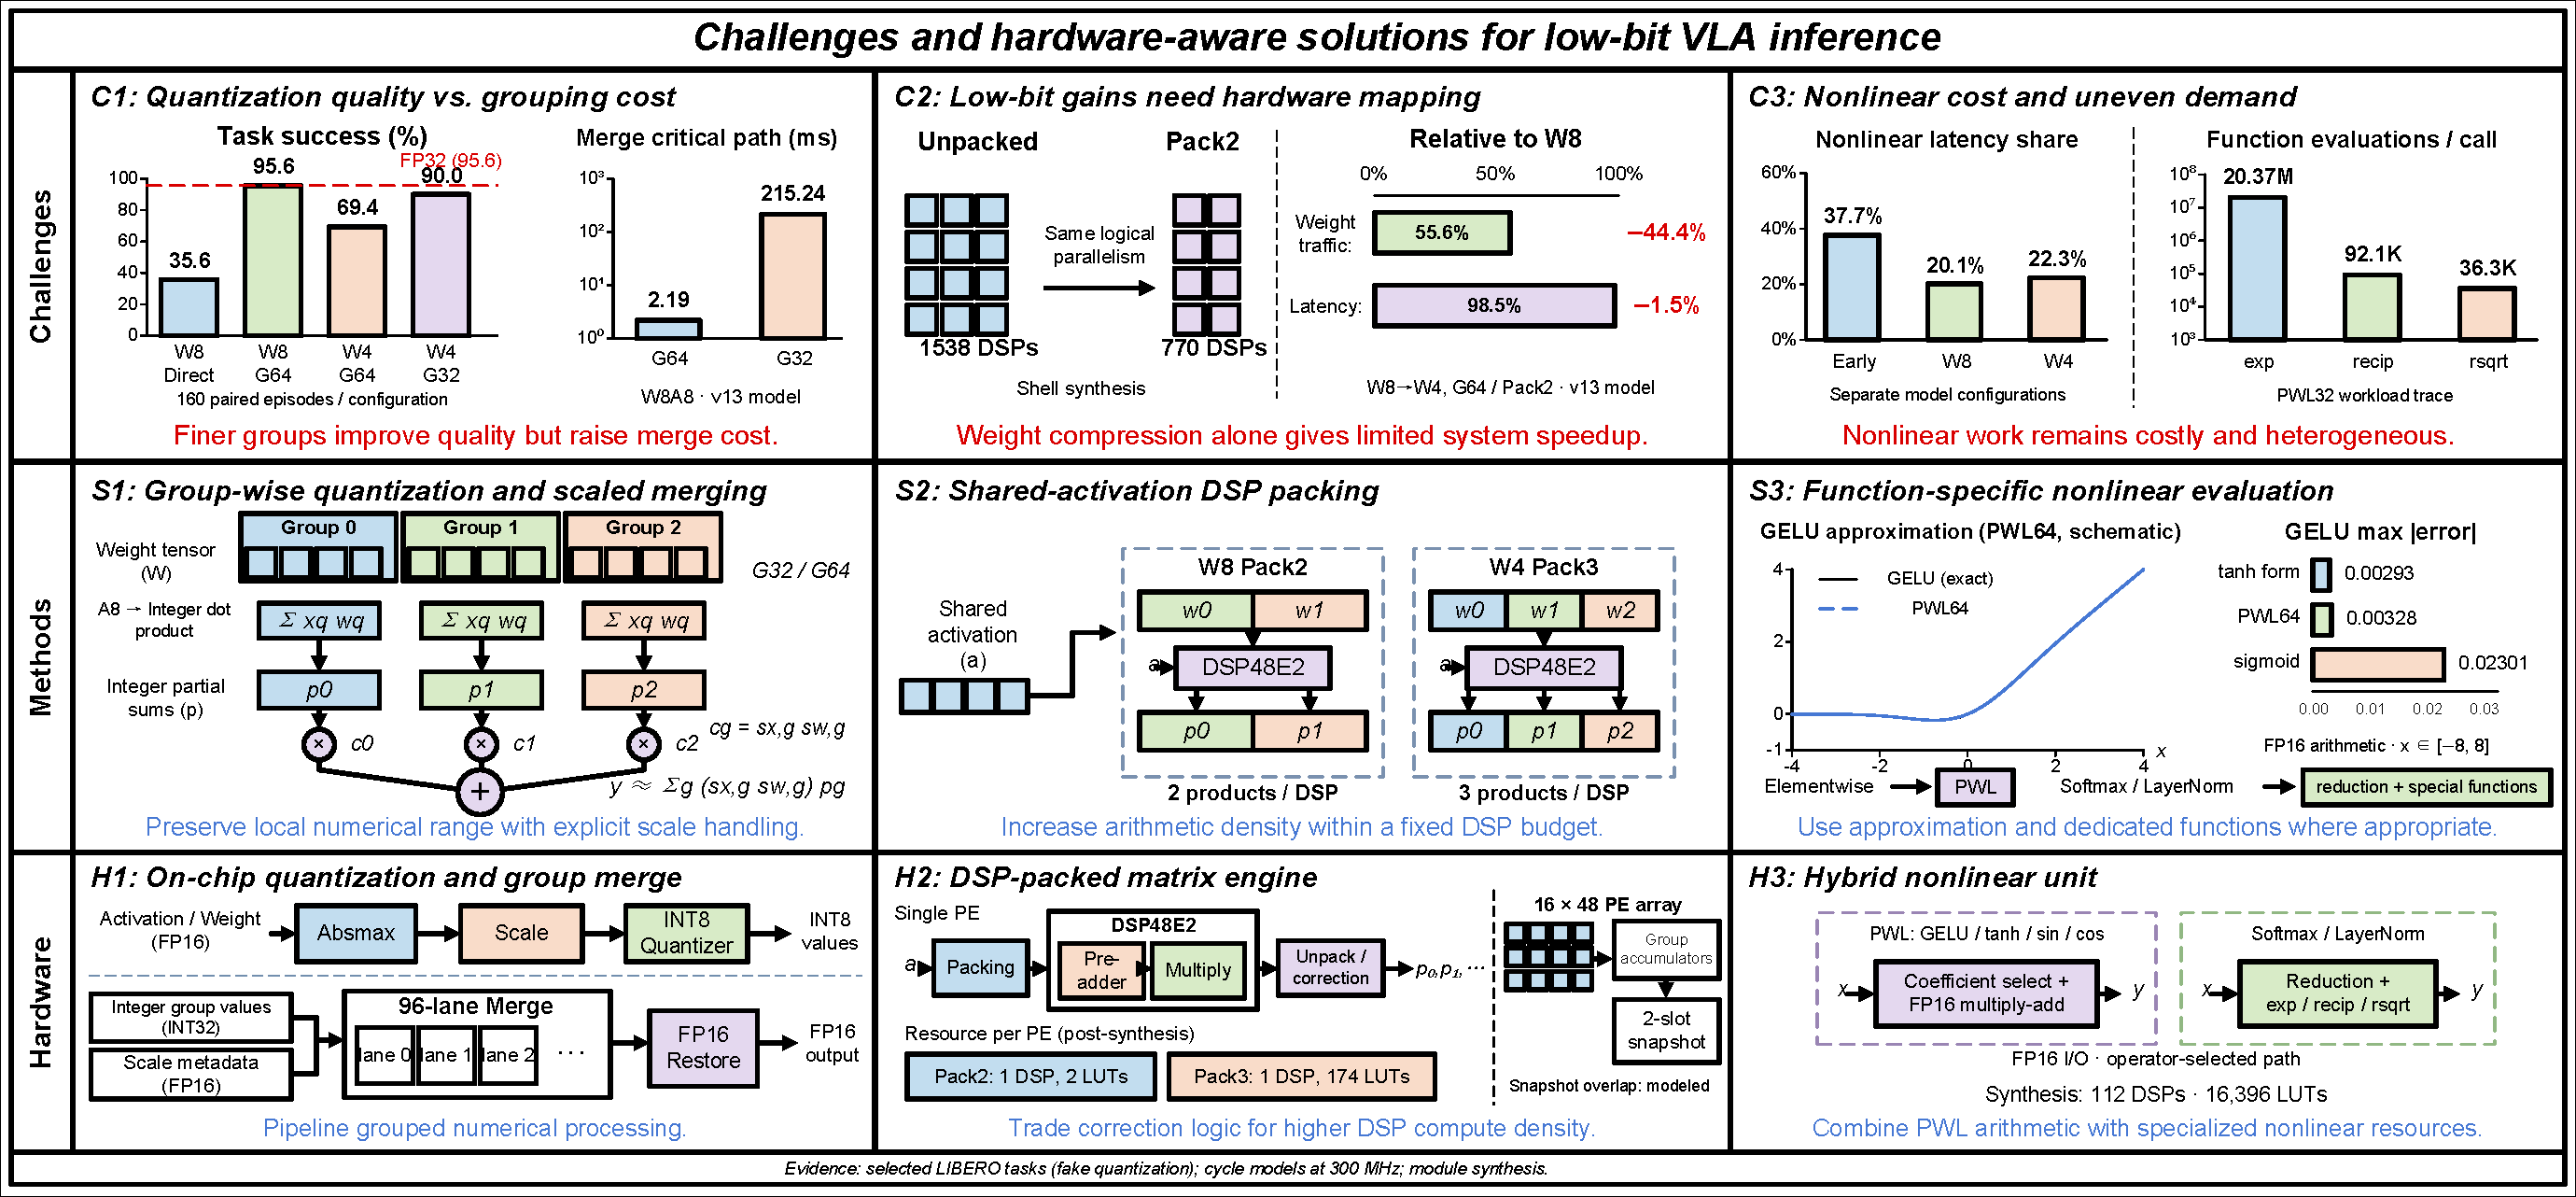
\includegraphics[width=.97\textwidth]{figures/narrative.pdf}
\caption{Workload challenges and hardware responses: C1/H1 quantization and merging, C2/H2 DSP-packed arithmetic, and C3/H3 nonlinear execution.}\label{fig:narrative}
\end{figure*}
Figure~\ref{fig:narrative} connects the workload observations to the hardware responses. The three challenges concern successive parts of one computation: representing inputs, producing integer products, and processing results and nonlinear operators. The design coordinates the service rates and buffering of these stages.

\section{Numerical Method and Arithmetic Mapping}\label{sec:method}
\subsection{Group-wise INT8 representation}
Let $A\in\mathbb{R}^{M\times K}$ and $B\in\mathbb{R}^{K\times N}$. For output indices $m,n$ and reduction group $g$, define $\mathcal{K}_g$ as the set of reduction indices in that group. For a vector $x$ and bit width $b$, the numerical reference uses
\begin{align}
L_b&=2^{b-1}-1,\\
s_x&=\max(\max_i|x_i|,\epsilon)/L_b,\\
q_i&=\operatorname{clip}(\RNE(x_i/s_x),-L_b,L_b),
\end{align}
where $\epsilon=10^{-12}$ in the software reference and RNE denotes round-to-nearest with ties to even. The W8A8 datapath uses $b=8$ and $L_8=127$ for weights and activations. Zero groups encode to zero.

The group product and its scale are
\begin{align}
p_{mng}&=\sum_{k\in\mathcal{K}_g}q^A_{mkg}q^B_{kng},\\
s_{mng}&=s^A_{mg}s^B_{ng},\\
Y_{mn}&\approx\sum_g s_{mng}p_{mng}.\label{eq:group}
\end{align}
Equation (\ref{eq:group}) uses row-, column-, and group-dependent scales. Padding a final incomplete group with zeros preserves the matrix dimensions after the padded positions are discarded.

\begin{figure}[t]\centering
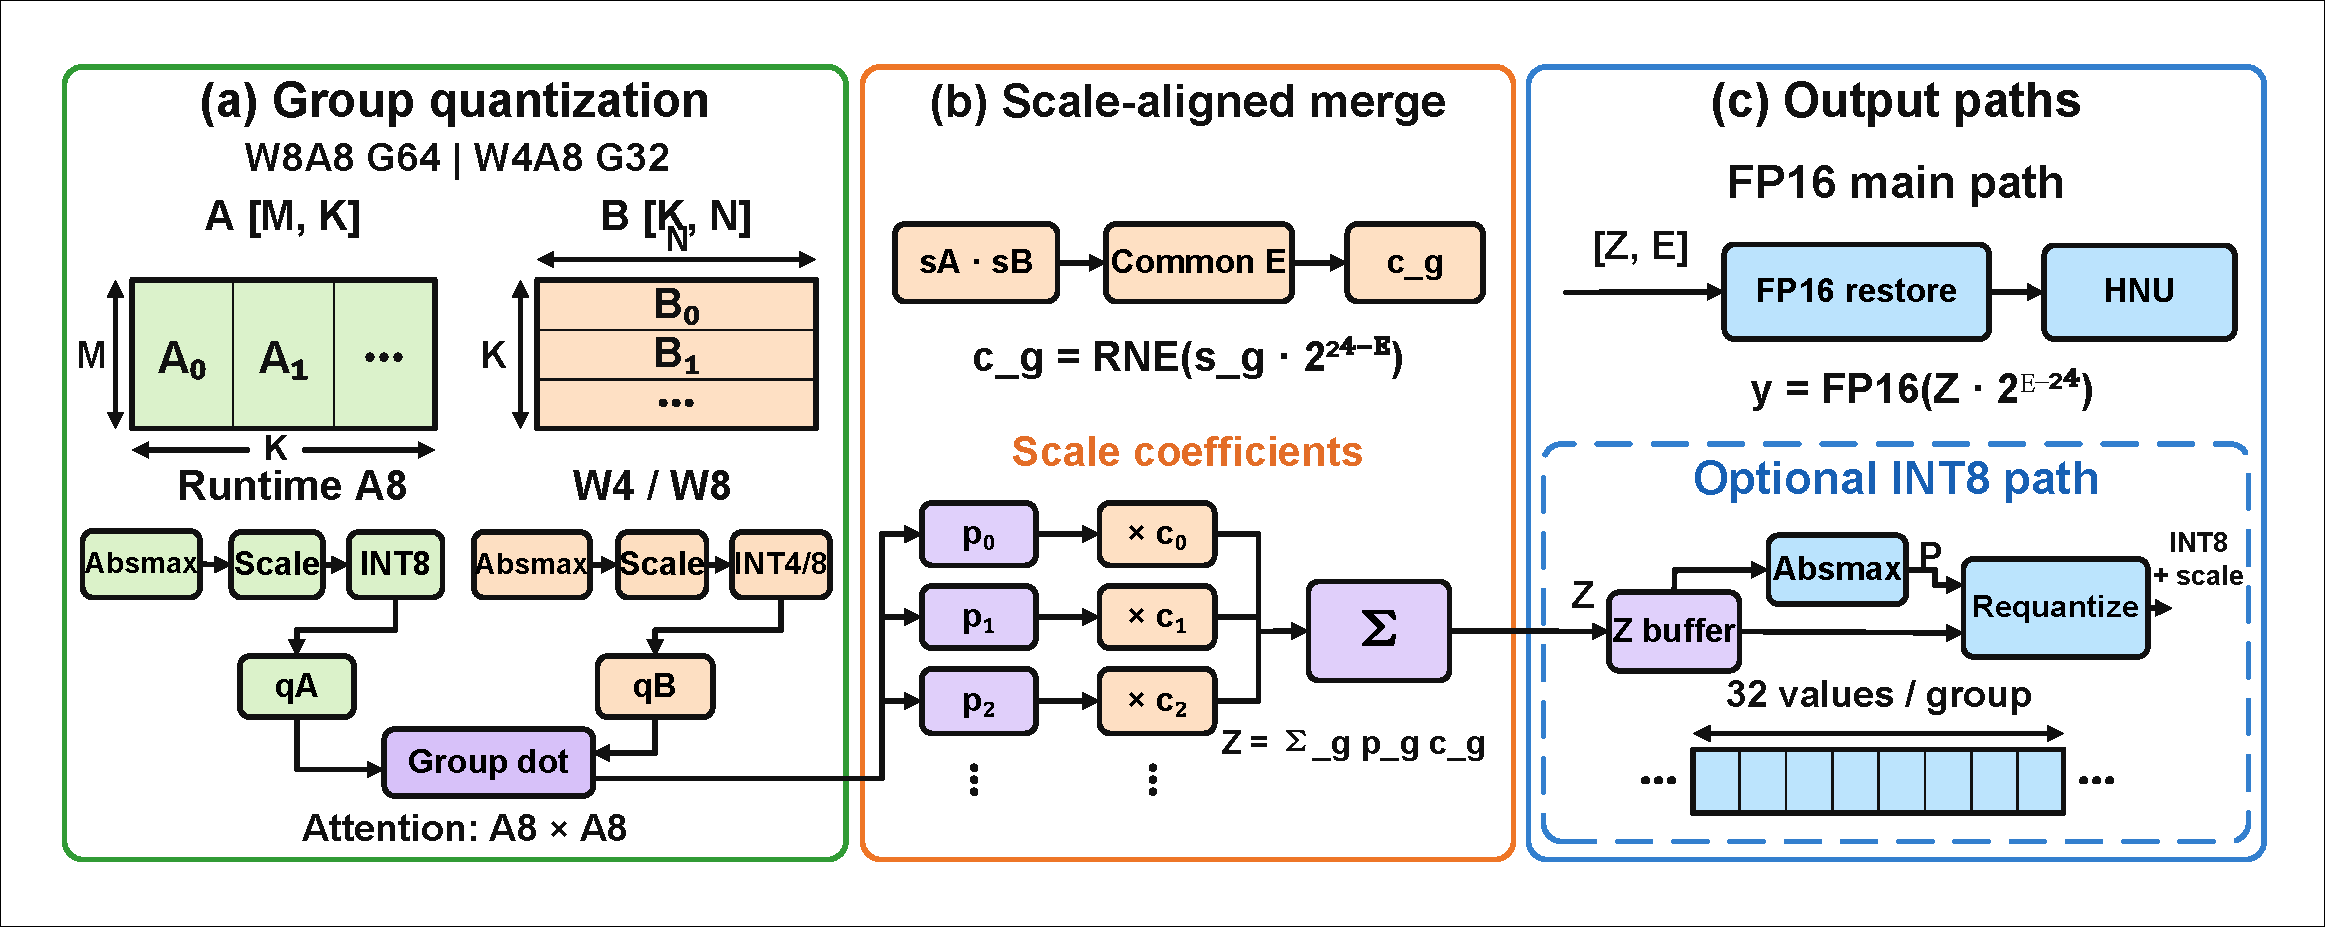
\includegraphics[width=\columnwidth]{figures/quantization.pdf}
\caption{H1 group-wise quantization algorithm. Inputs are grouped along $K$, group products are merged with aligned coefficients, and the output enters either FP16 restoration or integer re-encoding.}\label{fig:quant}
\end{figure}

\subsection{Common-exponent scale alignment}
Figure~\ref{fig:quant} separates integer products from scale metadata. A common exponent $E$ permits group scales to be represented as integer coefficients. The software reference obtains $E$ from the \texttt{frexp} exponent of the maximum scale product in the operation and forms
\begin{align}
c_{mng}&=\RNE(s_{mng}2^{24-E}),\\
Z_{mn}&=\sum_g p_{mng}c_{mng},\label{eq:merge}\\
\widehat Y_{mn}&=Z_{mn}2^{E-24}.
\end{align}
The exponent is retained with the result. Coefficients must be available before their corresponding partial sums are consumed. This preparation is distinct from the dot product itself, allowing the architecture to schedule scale handling separately from matrix arithmetic.

This representation introduces a coefficient-rounding error in addition to operand quantization. Before considering accumulator overflow, the coefficient contribution is bounded by
\begin{equation}
\left|\sum_g p_g(s_g-c_g2^{E-24})\right|
\leq 2^{E-25}\sum_g|p_g|.
\end{equation}
This coefficient-error bound follows from nearest rounding and determines the required exponent, coefficient range, and integer accumulation width.

The quality evaluation accumulates (\ref{eq:merge}) in INT64. The implemented merge primitive accepts a signed 17-bit dot product and a signed 24-bit coefficient, and accumulates in 48 bits. Mapping the reference computation to this interface requires range adaptation for group sums and coefficients; a full W8 G64 dot product can exceed the signed 17-bit input range.

\subsection{Output representation}
The FP16 path restores the common scale and rounds once to binary16:
\begin{equation}
y_{mn}=\operatorname{FP16}(Z_{mn}2^{E-24}).
\end{equation}
The dequantization RTL normalizes the integer magnitude, forms the exponent, and uses guard, round, and sticky information for nearest-even rounding. It handles normal and subnormal outputs, signed zero, and overflow to infinity. FP16 results can then enter vector operations and the HNU without inserting an INT8 re-encoding stage.

The optional integer stream instead buffers $Z$ and performs two passes. The first obtains the maximum magnitude $P_h$ within output group $h$. The second computes
\begin{equation}
q_h=\RNE(127Z_h/P_h),\qquad
s_h^{\rm out}=\frac{P_h}{127}2^{E-24}.
\end{equation}
A zero group produces zero output. Ordinary matrix outputs use 32-value groups along each output row. The action projection groups along time for the seven action coordinates. The second pass needs both the buffered values and their group maximum; it cannot be implemented from the maximum alone.

\subsection{Pack2: two signed W8A8 products}
Let signed eight-bit weights $w_0,w_1$ share a signed activation $a$. Offset encoding changes each weight to a nonnegative byte, implemented by flipping its sign bit. The packed word is
\begin{equation}
Q=(w_1+128)2^{16}+(w_0+128).
\end{equation}
The DSP pre-adder subtracts the constant $128(2^{16}+1)=8{,}388{,}736$ before multiplication, yielding
\begin{equation}
R=w_1 2^{16}+w_0,\qquad P=aR.
\end{equation}
This placement removes the activation-dependent offset correction from the post-multiply path. Signed products are recovered as
\begin{align}
p_0&=\operatorname{signed}(P[15:0]),\\
p_1&=\operatorname{signed}(P[31:16])+P[15].
\end{align}
The additional bit in $p_1$ corrects the borrow caused by a negative lower field. Omitting it would couple the numerical interpretation of the high field to the sign of the low product.

Pack2 uses one DSP per packed multiplier. Signed-product recovery feeds the downstream group accumulators.

\subsection{Nonlinear numerical paths}
For a piecewise-linear (PWL) function, interval selection returns a slope $\alpha_j$ and intercept $\beta_j$, and the elementwise path computes $f(x)\approx\alpha_jx+\beta_j$. The HNU uses a 64-segment organization for supported functions. Sharing the multiply-add structure across functions reduces duplicated arithmetic, while coefficient tables select the function-specific approximation.

Softmax and LayerNorm additionally require reductions. A stable Softmax implementation forms a row maximum, evaluates exponentials of shifted inputs, sums them, and multiplies by the reciprocal sum. LayerNorm computes normalization statistics and uses reciprocal square root. The architecture retains FP32 reduction state and FP16 interfaces, with distinct resources for these special functions.

\section{FPGA Architecture}\label{sec:architecture}
\subsection{Dataflow overview}
The architecture follows the numerical dependencies in Section~\ref{sec:method}. DMA transfers inputs and parameters between external memory and on-chip banks. Runtime quantization produces grouped activation records. The matrix array consumes quantized operands, and group results enter snapshot storage before scale-aligned merging. The completed result is restored to FP16 for vector and nonlinear processing, or encoded for a compatible integer consumer.

\begin{figure}[t]\centering
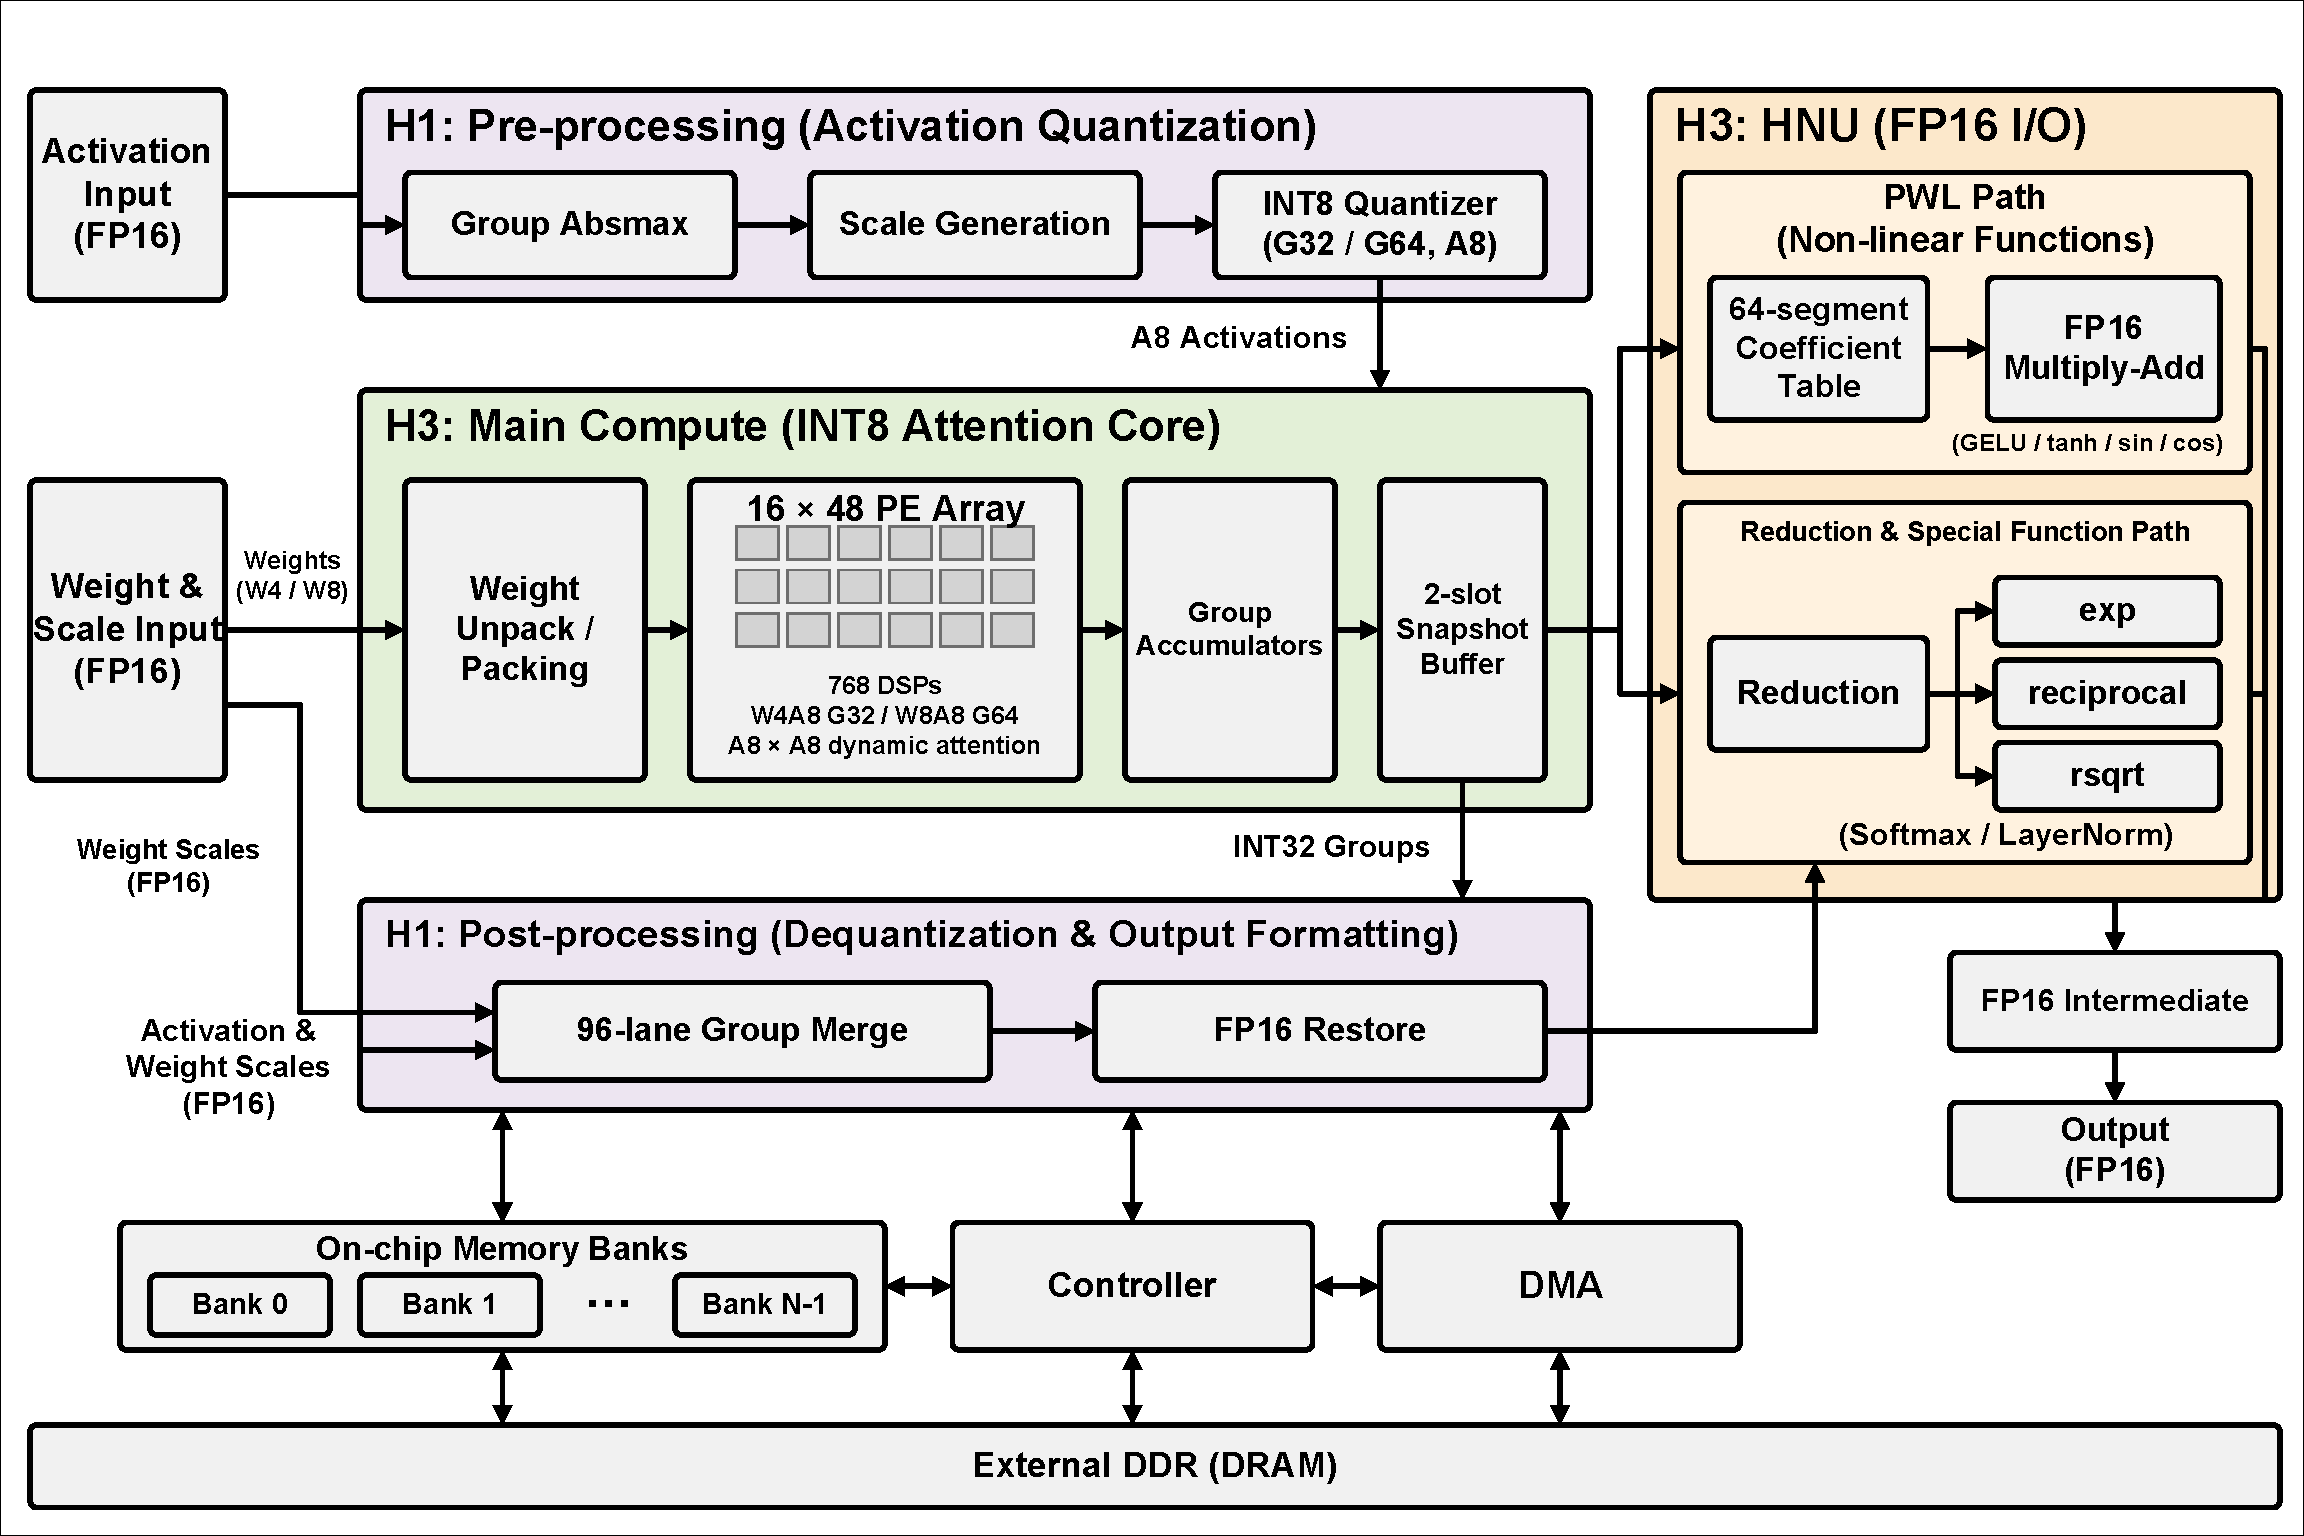
\includegraphics[width=\columnwidth]{figures/architecture.pdf}
\caption{Vela architecture. H1 performs input quantization and group merging, H2 executes packed matrix arithmetic, and H3 handles nonlinear and reduction operations. Scale restoration supplies FP16 consumers with merged results.}\label{fig:architecture}
\end{figure}

Figure~\ref{fig:architecture} provides the module-level view. Compiler-generated execution plans supply operator order, addresses, grouping, and output-format choices. The controller coordinates these decisions rather than introducing another numerical approximation. Read ports and a DMA path support overlap between data movement and execution where dependencies permit it. Resource availability and buffer ownership remain explicit constraints on that overlap.

\subsection{H1: Runtime quantization}
The activation quantizer processes 32 FP16 values per input beat. G32 forms one group from one beat; G64 forms a group from two consecutive valid beats. Group absmax determines shared parameters, while elementwise pipelines produce signed INT8 values. The G64 pair must arrive consecutively within a group, although idle cycles are allowed between groups.

\begin{figure}[t]\centering
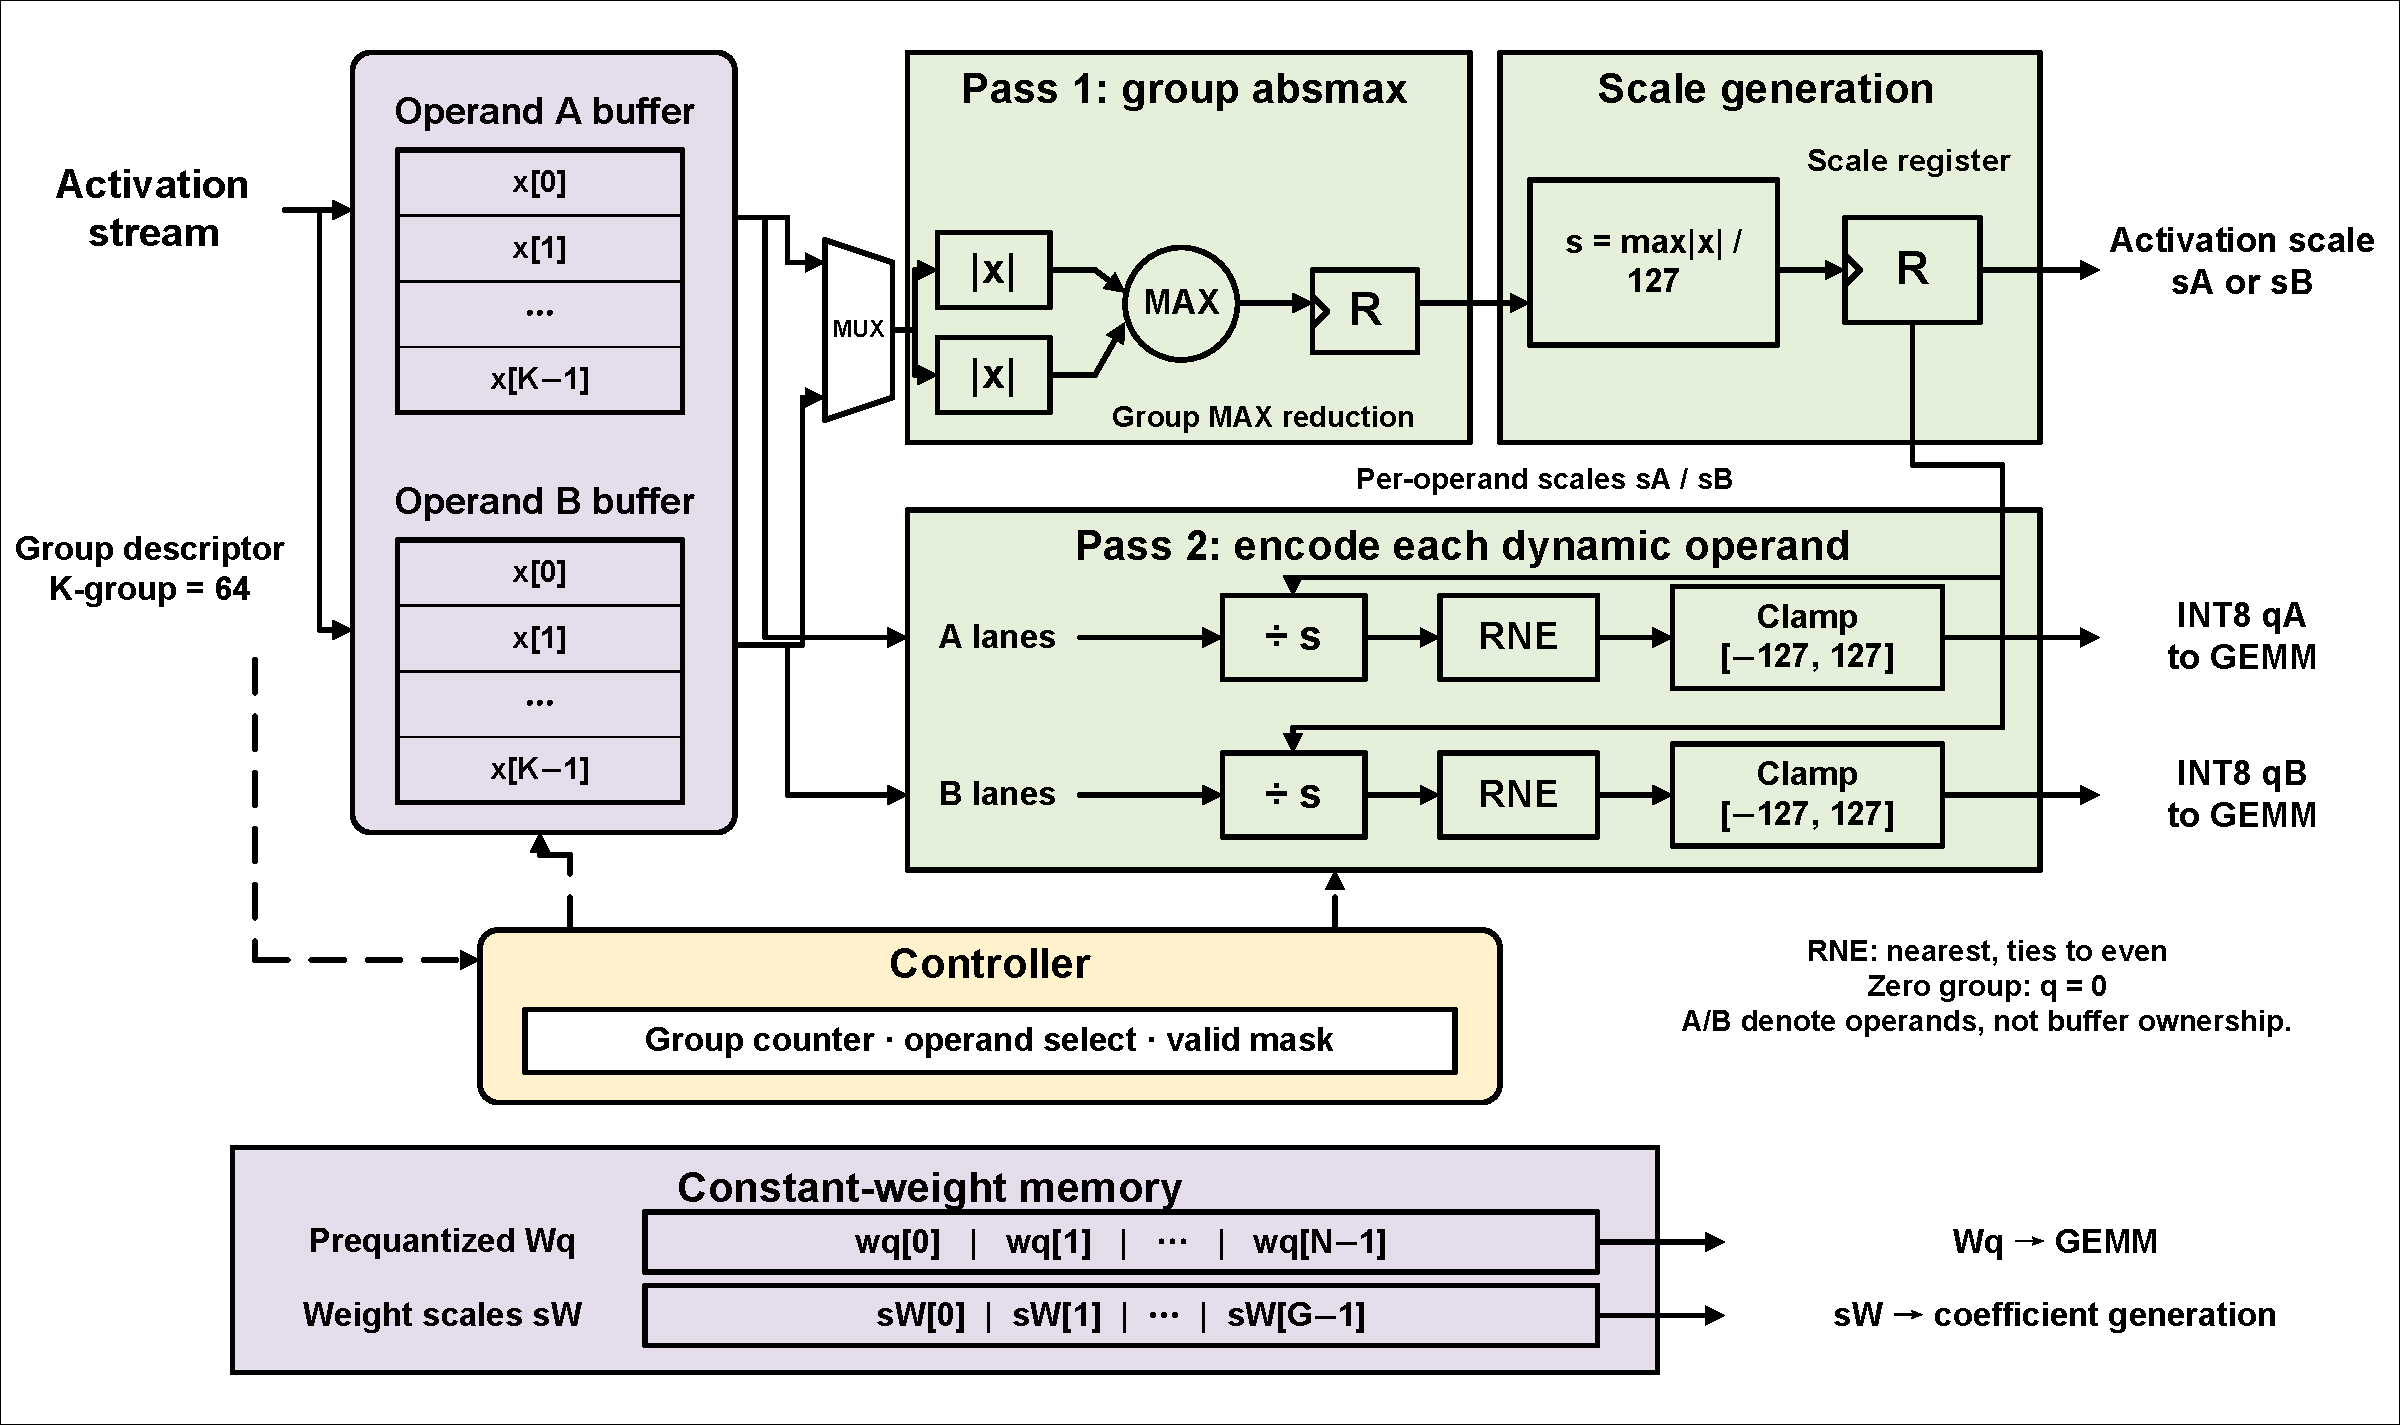
\includegraphics[width=\linewidth]{figures/input_quant.pdf}
\caption{Input quantization datapath. The parameterized implementation supports G32 and G64 at 32 FP16 input values per beat.}\label{fig:input}
\end{figure}

Figure~\ref{fig:input} separates group statistics from element processing. The implementation uses reciprocal-related parameters and integer correction to reproduce the reference rounding behavior, including half-integer cases. Parameters and element data travel through aligned pipelines so that every quantized value uses its own group's maximum.

The output record contains $G$ quantized bytes and an eight-byte descriptor. The record sizes are therefore 40 bytes for G32 and 72 bytes for G64. Relative to two-byte FP16 input values, these correspond to 37.5\% and 43.75\% smaller activation records, respectively, before considering other transfers or buffering. The larger metadata fraction at G32 illustrates a second cost of fine grouping beyond the number of group results.

\subsection{H1: Snapshots and 96-lane merging}
The architecture model places two snapshot slots between group-result production and merge consumption. A completed group can occupy one slot while the merger consumes the other. The intended ownership rule is that the array writes only a free slot and the merger reads only a completed slot. A slot becomes reusable after its results have been consumed. If both slots are occupied, production must wait.

Let $T_p$ denote the average production interval and $T_m$ the time needed to consume a group snapshot. Sustained overlap requires $T_m\leq T_p$; otherwise the two slots eventually fill and backpressure stalls production. This service-rate condition motivates the 96-lane merge width. The cycle-level scheduler tracks slot ownership and backpressure explicitly.

\begin{figure}[t]\centering
\includegraphics[page=2,width=\columnwidth]{figures/pe_merge.pdf}
\caption{Updated merge96 datapath. Each lane receives its own dot product and coefficient. Coefficient concatenation precedes multiplication; the lane then performs one DSP multiply--accumulate into a signed 48-bit result.}\label{fig:merge}
\end{figure}

Figure~\ref{fig:merge} shows the implemented merge primitive. Split coefficient metadata contains signed high bits $h$ and unsigned low bits $l$. Their reconstruction is
\begin{equation}
C_q=64h+l=\{h,l\}.
\end{equation}
Because the fields do not overlap, concatenation implements the reconstruction without an adder. This moves the split from the multiplication side to the coefficient side. Each lane then fits a 24-by-17-bit product and 48-bit accumulation into one DSP.

The lane's registered valid signal enables an update. Its clear signal selects zero instead of the previous accumulator, while still adding the current product. Invalid cycles hold the accumulator. A 96-lane instance broadcasts valid and clear but retains independent data and coefficients for each lane. The earlier split-multiplication implementation used 288 DSPs; coefficient-side reconstruction uses 96, a 66.7\% reduction for this module.

\subsection{H2: Packed arithmetic and array organization}
Figure~\ref{fig:pe} shows the Pack2 mapping to the DSP48E2 pre-adder and multiplier. Pack2 accepts two offset W8 fields and the sign-extended A8 operand. The DSP output is registered, with control information delayed alongside the data before signed-product recovery and group accumulation.

\begin{figure}[t]\centering
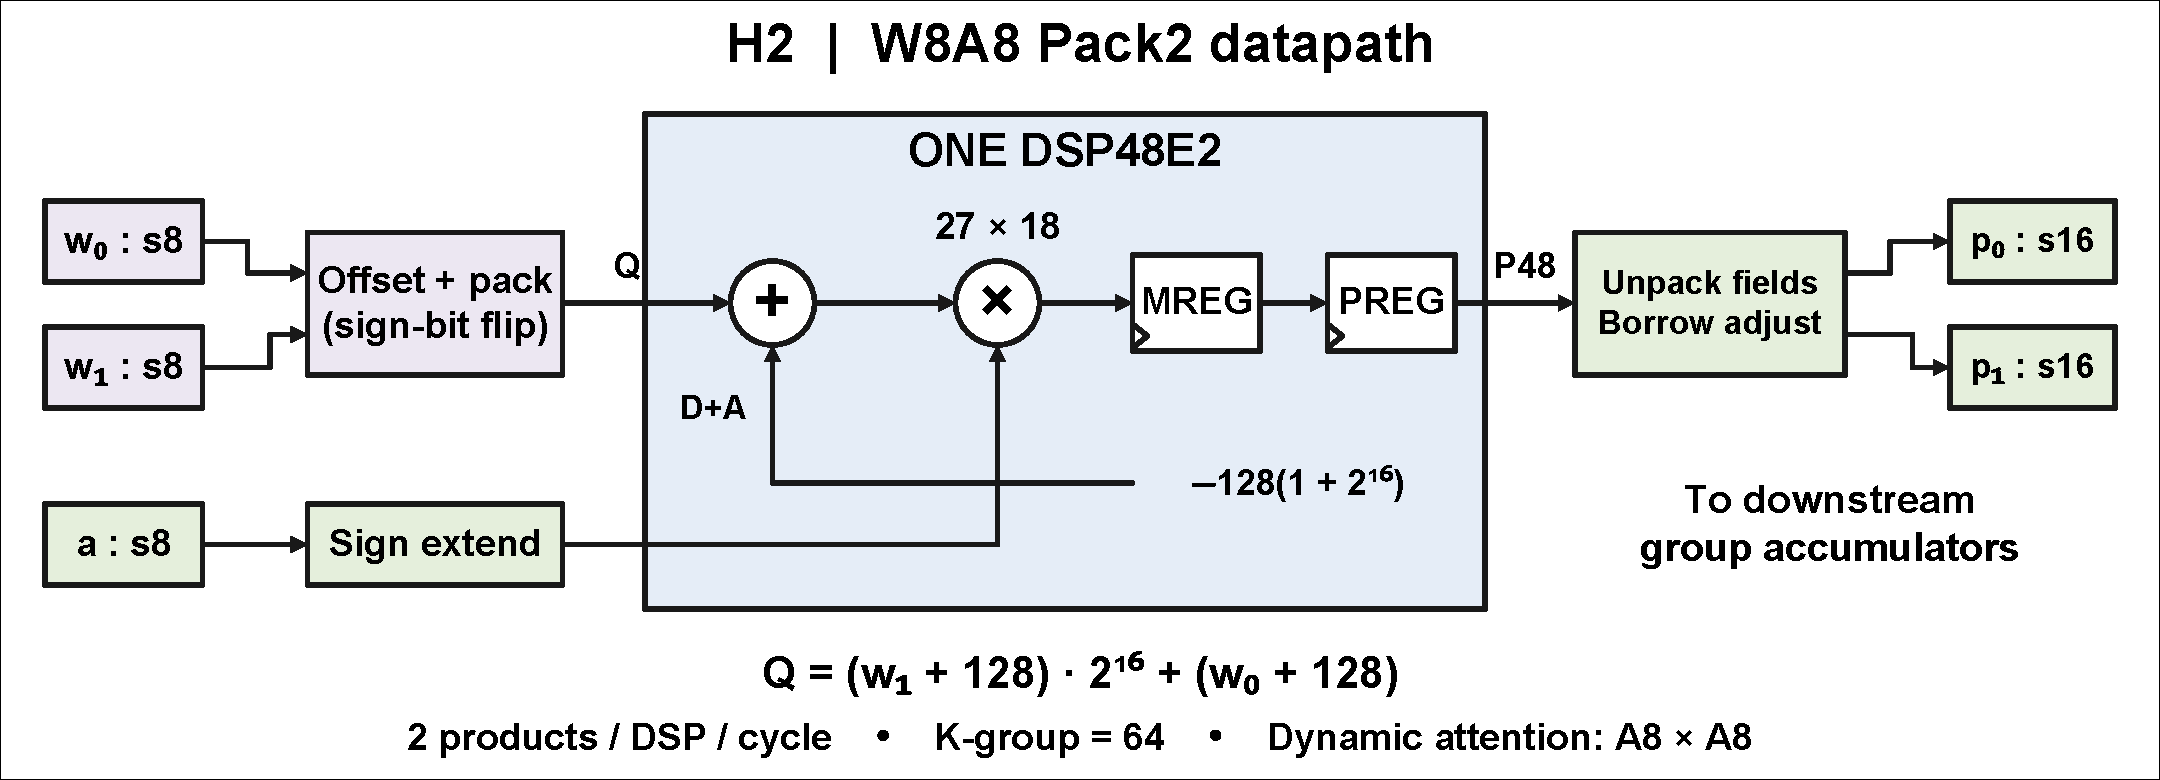
\includegraphics[page=1,width=\columnwidth]{figures/pe_merge.pdf}
\caption{H2 Pack2 circuit datapath. Two separate W8 operands share an A8 input. The DSP pre-adder removes the packing offset before multiplication; MREG and PREG register the packed result. Field extraction recovers two signed products for downstream group accumulation.}\label{fig:pe}
\end{figure}

The matrix architecture uses a $16\times48$ physical PE organization with 768 matrix DSPs. Pack2 provides 96 logical columns. Output tiling and scheduling determine how group results enter the snapshot slots and 96 merge lanes.

Dynamic attention uses the same Pack2 arithmetic for A8-by-A8 products. Its operands are quantized at runtime, while static W8 parameters can be prepared offline. Both feed the shared group-result and scale-aligned merge path.

\subsection{H3: Heterogeneous nonlinear execution}
The HNU divides its work between a 32-lane shared elementwise path, FP32 reductions, and special-function units, as shown in Fig.~\ref{fig:hnu}. A 64-segment coefficient table supplies the slope and intercept for PWL evaluation. The elementwise lanes reuse multiply-add arithmetic across supported nonlinear functions.

\begin{figure}[t]\centering
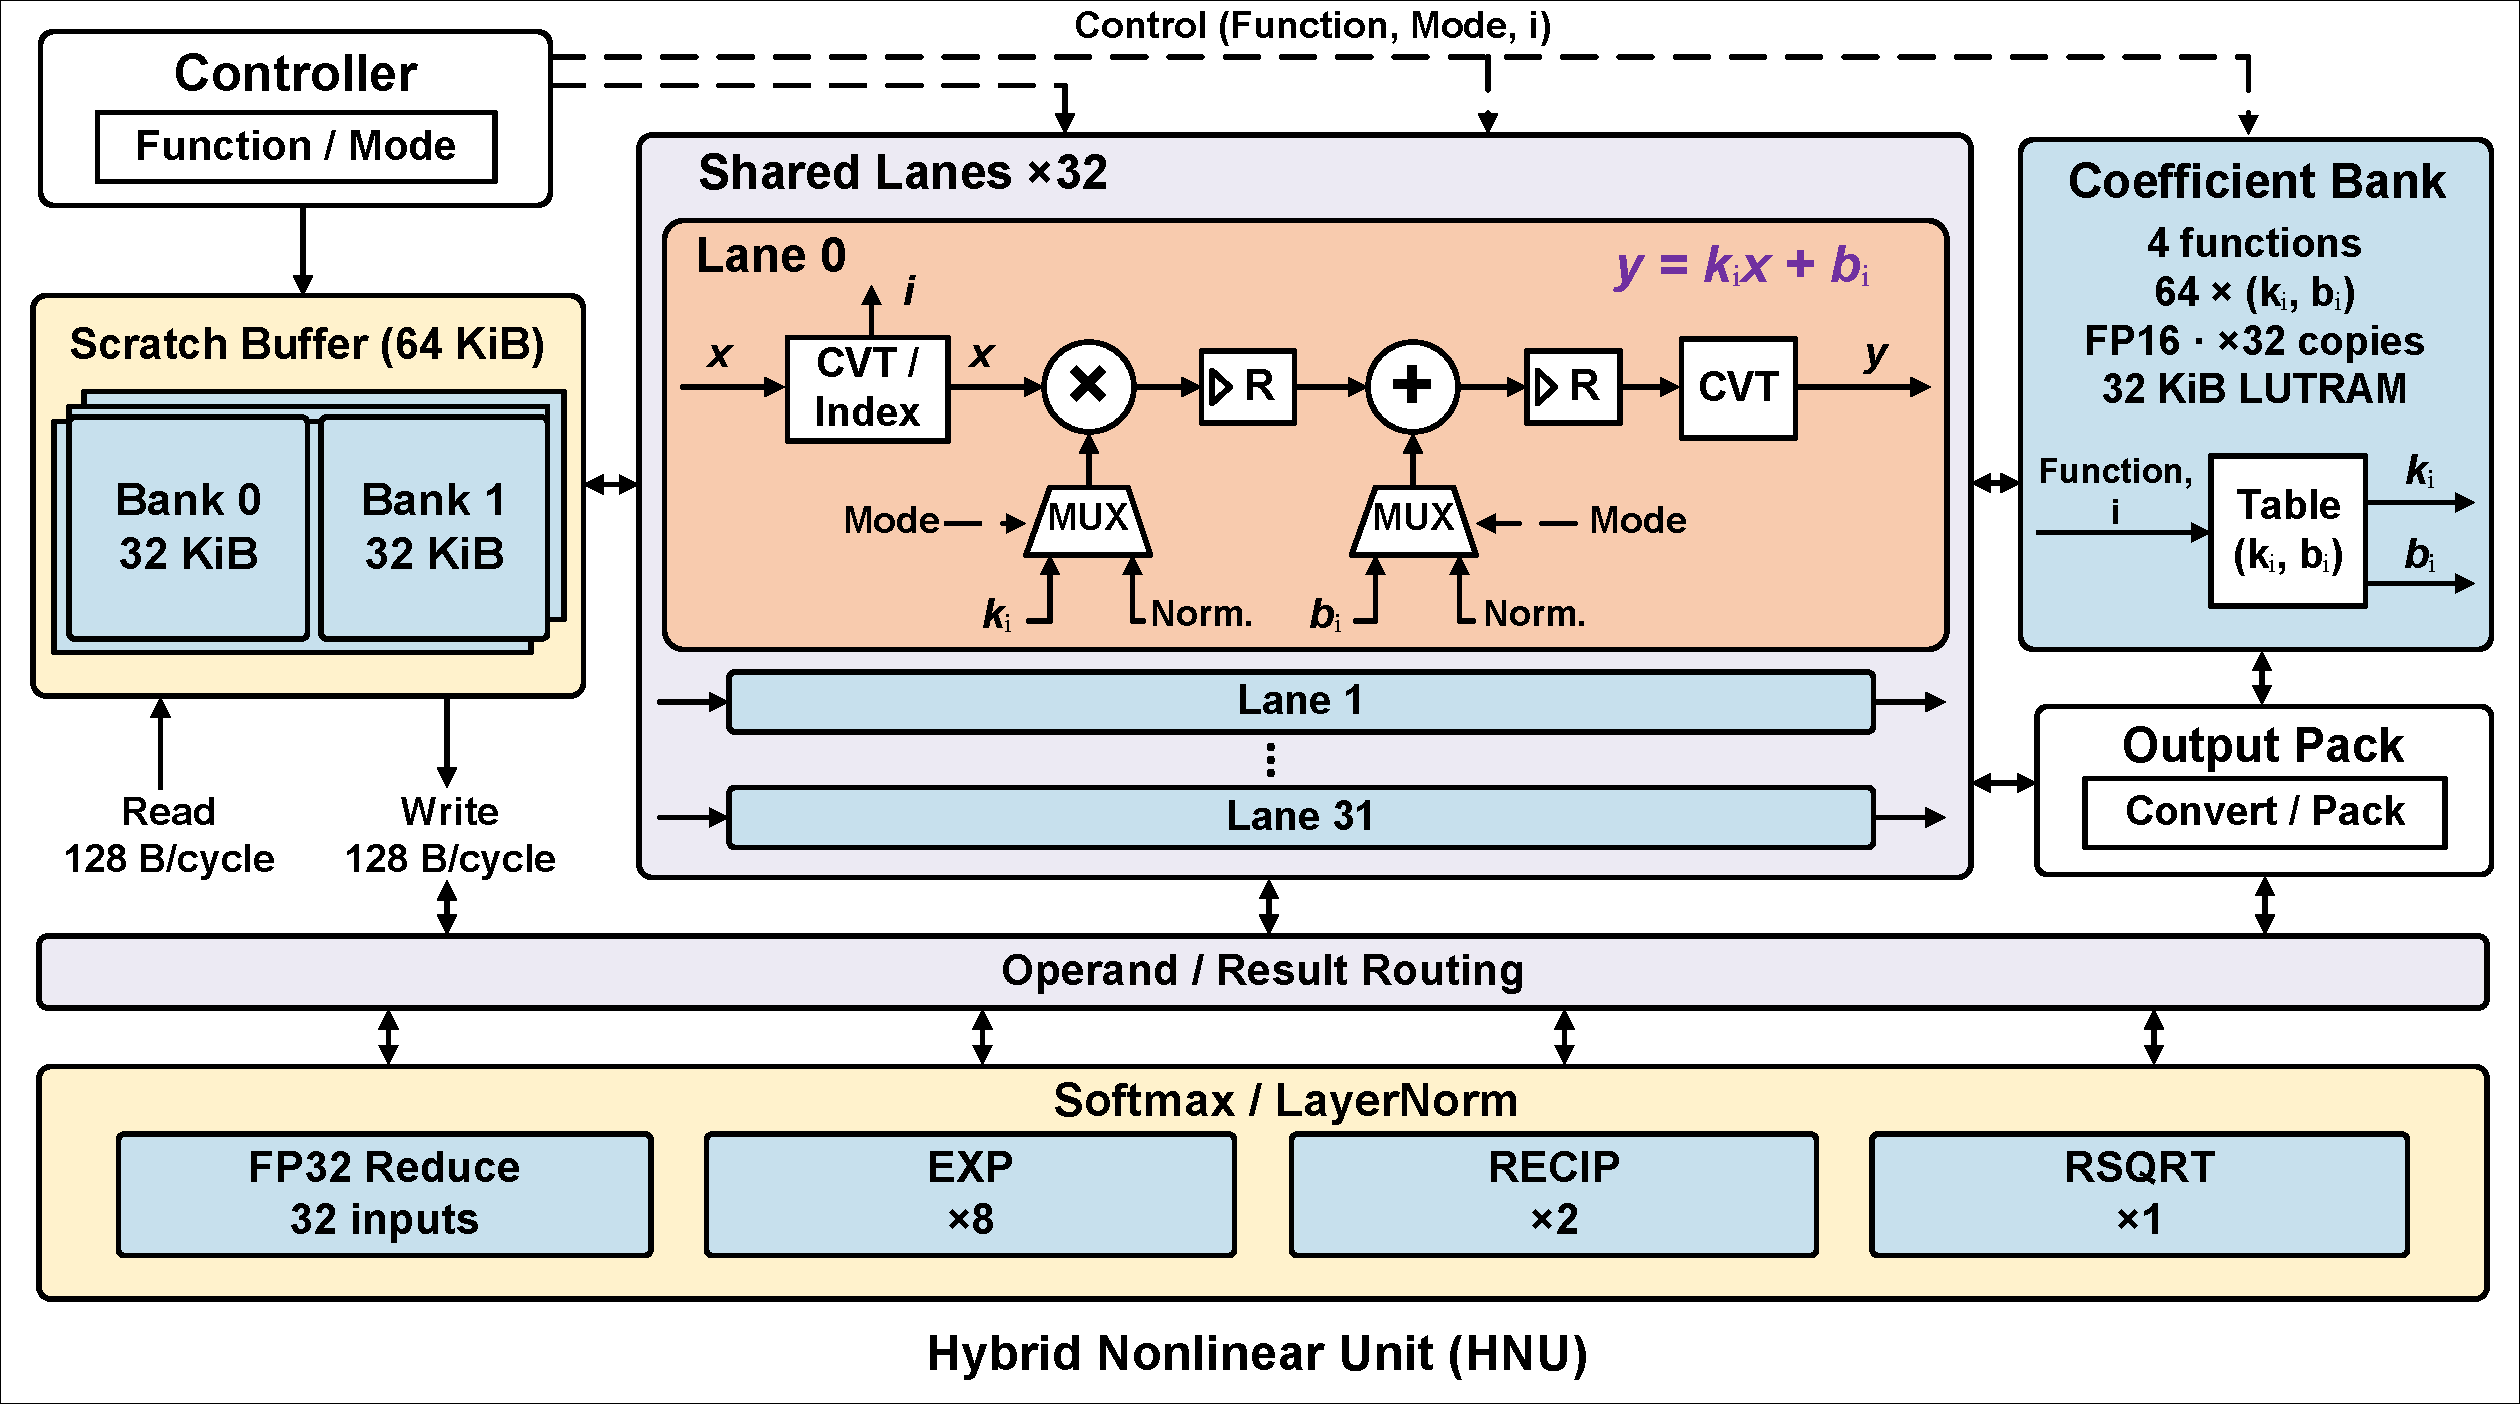
\includegraphics[width=\columnwidth]{figures/hnu.pdf}
\caption{HNU datapath with 32 shared PWL lanes, FP32 reduction state, eight exponential units, two reciprocal units, and one reciprocal-square-root unit.}\label{fig:hnu}
\end{figure}

The special-function mix reflects differing service demands. Exponentials are consumed across Softmax elements, whereas reciprocal and reciprocal-square-root results are shared by a normalized row. The architecture therefore allocates more lanes to exponential evaluation than to row-level reciprocal operations.

Reduction state accumulates values across a row before dependent operations are released. The row maximum and sum in Softmax, for example, determine when exponentiation and normalization can proceed. The controller must preserve these dependencies even when independent elementwise work is available. This is the reason H3 includes both arithmetic paths and scheduling state, rather than a single lookup-and-multiply block.

\subsection{Memory and execution control}
Grouped data records couple values with descriptors, allowing consumers to identify group boundaries and interpret scales. The controller associates each scheduled operation with its input representation and selected output path. Buffers cannot be reused simply because a matrix tile has finished computing: snapshots, coefficient consumers, and vector operations may still reference their contents.

Read arbitration, local movement, and DMA resources track these data dependencies. The execution schedule overlaps data transfers with arithmetic and attributes invocation cycles to the critical path.

\section{Evaluation}\label{sec:eval}
\subsection{Experimental setup}
The quality study uses a fixed TurboVLA LIBERO checkpoint with EMA parameters and the \texttt{libero\_all4\_no\_noops} preprocessing statistics. It evaluates task indices 0 and 1 from each of the LIBERO Spatial, Object, Goal, and Long suites~\cite{libero}, using initial states 3--22 and seed $7+\text{state\_id}$. Each configuration is evaluated on 160 episodes across these eight tasks. Three successful W8 episodes illustrate the action sequences.

Closed-loop quality is measured with the software numerical implementation: Q24/INT64 merging, nearest-even output encoding, and floating-point auxiliary operations. The Direct configuration changes scale granularity while keeping the evaluation protocol fixed. Hardware evaluation covers the FP16 restoration, HNU, and merge primitives described in Sections~\ref{sec:method} and~\ref{sec:architecture}.

Latency is evaluated using a cycle-level event model of the 2,277-operator W8A8 G64 invocation at 300 MHz. Module resources, timing, and power are obtained with Vivado 2021.2 on an \texttt{xczu7ev-ffvc1156-2-e} device. Each module undergoes out-of-context synthesis, optimization, placement, physical optimization, and routing under a 3.333 ns clock constraint. This flow characterizes individual modules before top-level clock-tree integration.

Power uses post-route vectorless activity estimation. The W8 multiplier wrapper covers 768 product cores and their input registers; downstream group accumulation lies outside this reported hierarchy. Aggregate estimates sum the listed modules with one G64 quantizer, one G32 output encoder, DMA included in the memory subsystem, and one device-static contribution. The ablation DSP budget comprises the matrix, merge, HNU, and controller resources; the module subtotal additionally includes 97 quantizer DSPs and one encoder DSP.

\subsection{Closed-loop quality}
Table~\ref{tab:quality} and Fig.~\ref{fig:quality} show the precision-group tradeoff. W8 G64 matches the FP32 total of 153 successes. W4 G32 reaches 144 successes, a reduction of 5.625 percentage points.

\begin{table}[t]\centering\small
\caption{Closed-loop quality across eight LIBERO tasks and 160 episodes.}\label{tab:quality}
\begin{tabular}{lrrr}\toprule
Configuration & Successes & Rate (\%) & $\Delta$ FP32 (pp)\\\midrule
FP32 &153&95.625&0\\
W8 Direct &57&35.625&$-60.000$\\
W8 G32 &151&94.375&$-1.250$\\
W8 G64 &153&95.625&0\\
W8 G128 &152&95.000&$-0.625$\\
W4 Direct &1&0.625&$-95.000$\\
W4 G32 &144&90.000&$-5.625$\\
W4 G64 &111&69.375&$-26.250$\\
W4 G128 &105&65.625&$-30.000$\\\bottomrule
\end{tabular}
\end{table}
\begin{figure*}[t]\centering
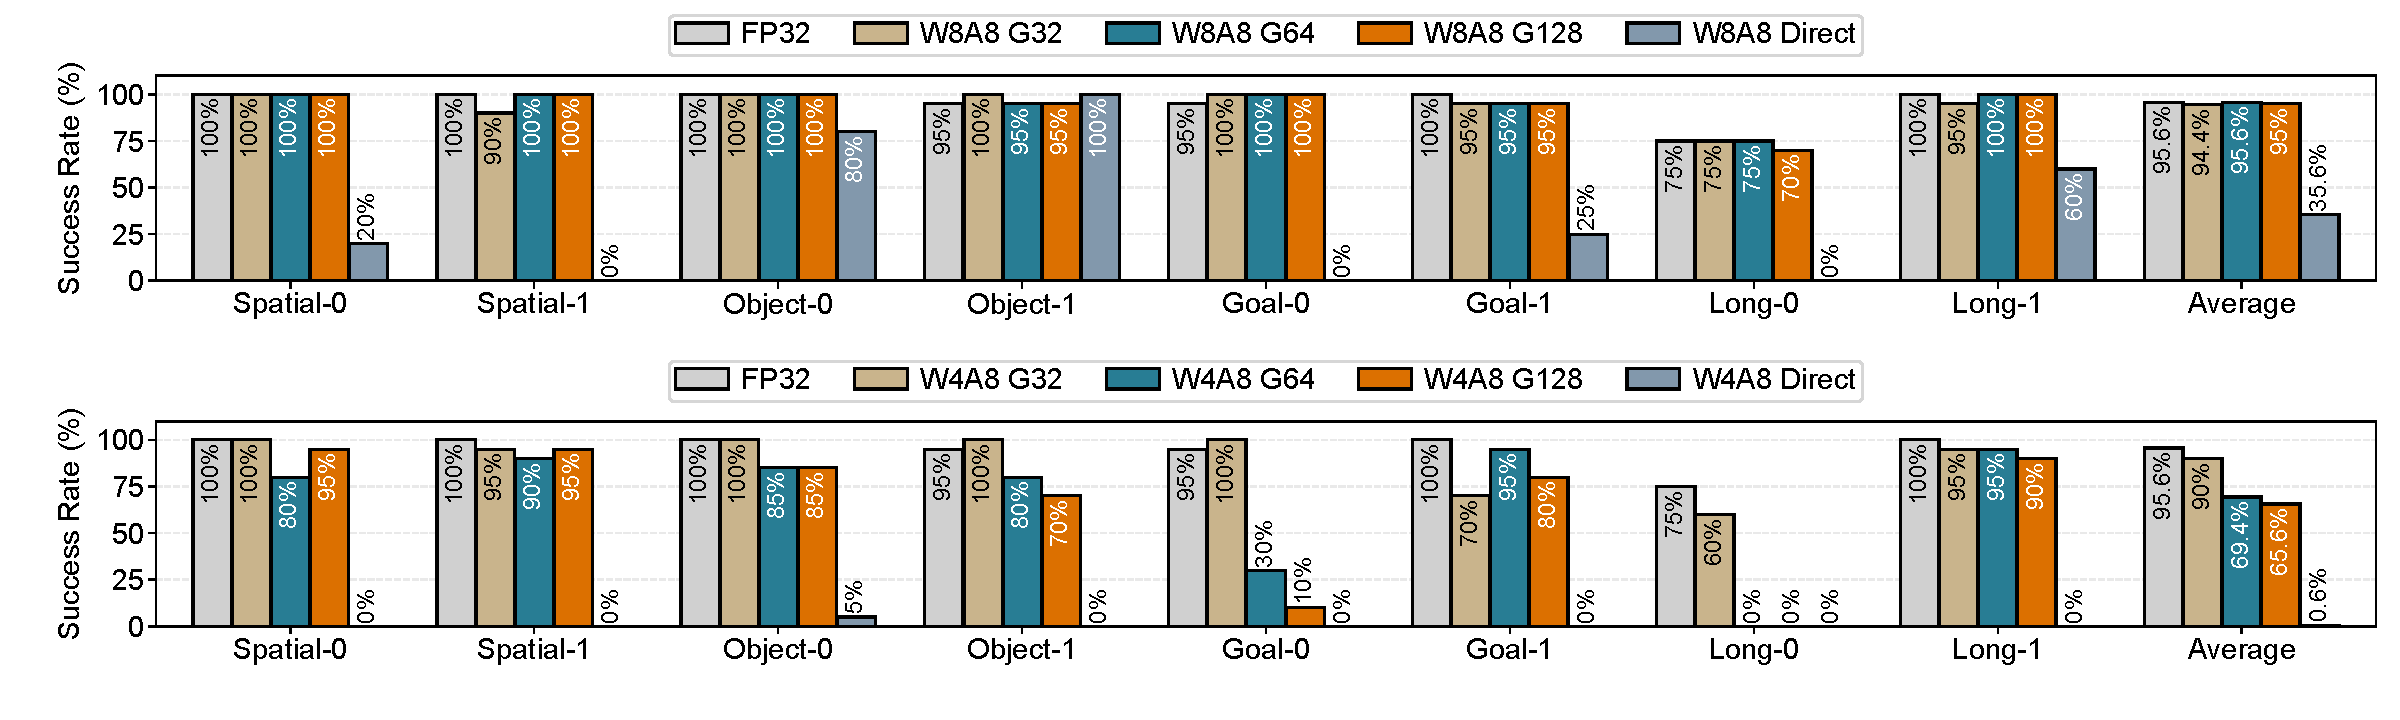
\includegraphics[width=.98\textwidth]{figures/quality.pdf}
\caption{Closed-loop success rates for different weight precisions and group sizes.}\label{fig:quality}
\end{figure*}

Fine grouping is particularly important for W4. Moving from G64 to G32 improves success by 20.625 percentage points, or 29.73\% relative to the G64 rate. W8 exhibits much smaller differences across the grouped configurations. Thus, using the same group size for both weight formats would hide a material part of the design space.

Task-level results further qualify the aggregate. Table~\ref{tab:tasks} shows that W4 G32 succeeds in all 40 Object episodes, but loses more episodes in Goal and Long tasks. An Object-only comparison would therefore overstate its quality across the selected workloads. The W8 operating point also exchanges successes between the two Goal tasks despite matching the floating-point aggregate.

\begin{table}[t]\centering\small
\caption{Successes per selected task; 20 episodes each.}\label{tab:tasks}
\begin{tabular}{lrrr}\toprule Task & FP32 & W8 G64 & W4 G32\\\midrule
Spatial 0 &20&20&20\\Spatial 1 &20&20&19\\
Object 0 &20&20&20\\Object 1 &19&19&20\\
Goal 0 &19&20&20\\Goal 1 &20&19&14\\
Long 0 &15&15&12\\Long 1 &20&20&19\\\bottomrule
\end{tabular}
\end{table}

Figure~\ref{fig:rollout} illustrates three successful W8 episodes, showing the policy-controlled sequence from initial observation to task completion in simulation.
\begin{figure}[t]\centering
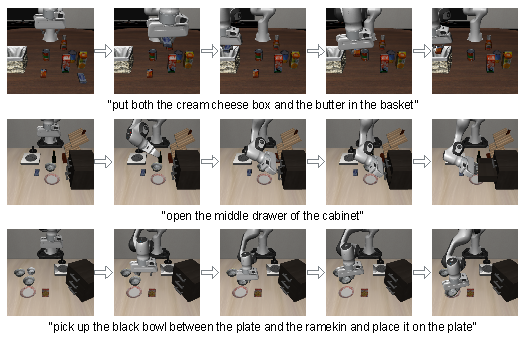
\includegraphics[width=\columnwidth]{figures/fig10_rollout_full_resolution.pdf}
\caption{Representative W8A8 G64 closed-loop rollouts in LIBERO simulation.}\label{fig:rollout}
\end{figure}

\subsection{Inference latency}
Table~\ref{tab:latency} reports the complete W8A8 G64 invocation schedule: 128,304,013 cycles, or 427.680 ms at the model clock. The schedule includes data movement, group processing, and nonlinear computation in addition to packed multiplication.

\begin{table}[t]\centering\small
\caption{W8A8 G64 inference latency at 300 MHz.}\label{tab:latency}
\begin{tabular}{lr}\toprule Metric & W8 G64\\\midrule
Total cycles (million)&128.304\\
Latency (ms)&427.680\\
Nonlinear critical cycles (million)&25.834\\
Nonlinear critical share (\%)&20.14\\\bottomrule
\end{tabular}
\end{table}

Nonlinear operations account for 20.14\% of the critical-path cycles. Their service time remains an important optimization target alongside the matrix path, motivating the dedicated function resources in H3.

\begin{figure}[t]\centering
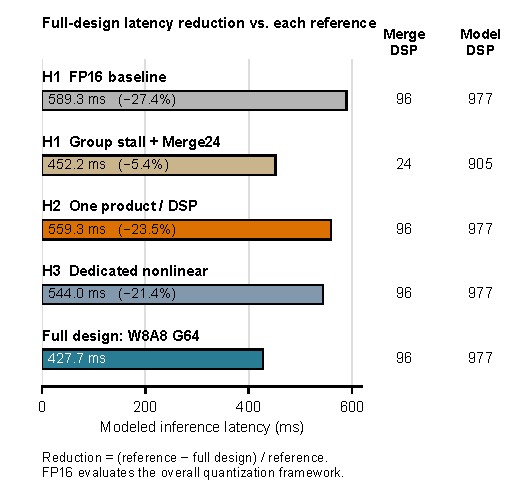
\includegraphics[width=\columnwidth]{figures/fig11_ablation.pdf}
\caption{Framework and mechanism comparisons at 300 MHz. Percentages denote full-design latency reductions relative to each row. H1 includes FP16 execution and group-stall/Merge24 references; H2 uses one product per DSP; H3 uses dedicated nonlinear units. DSP columns give merge resources and the ablation resource budget.}\label{fig:ablation}
\end{figure}

\subsection{Framework and mechanism comparisons}
Figure~\ref{fig:ablation} evaluates the complete design against four references in the cycle-level model. The comparisons use the same workload trace and memory configuration at 300 MHz. The FP16 reference changes the numerical representation and bypasses quantization; the three mechanism references retain W8A8 G64. Each reported reduction is $(T_{\mathrm{ref}}-T_{\mathrm{full}})/T_{\mathrm{ref}}$.

\textbf{H1: grouped quantization framework.} The matched-resource FP16 array reference requires 589.3 ms, compared with 427.7 ms for the complete W8A8 G64 design, a 27.4\% reduction. This comparison measures the overall benefit of quantized execution, including the packed arithmetic enabled by INT8 operands.

The second H1 reference removes double-buffered group snapshots, stalls the array at group boundaries, and reduces merge width from 96 to 24 lanes. Its latency is 452.2 ms, so the complete organization reduces latency by 5.4\%. The rollback uses 24 merge DSPs and reduces the ablation resource budget from 977 to 905 DSPs (7.4\%), exposing the latency--resource tradeoff. The overlap-only check retains Merge96 and takes 450.7 ms, corresponding to a 5.1\% full-design reduction; retaining snapshots with Merge24 takes 429.2 ms. These checks identify overlap as the main latency contributor at G64.

\textbf{H2: packed multiplication.} With one INT8 product per DSP cycle, invocation latency is 559.3 ms. Pack2 reduces this to 427.7 ms, a 23.5\% reduction under the same recorded DSP budget. This system improvement is smaller than the twofold product density because group processing, nonlinear execution, and data movement remain in the schedule.

\textbf{H3: shared nonlinear datapath.} The dedicated-function reference partitions the nonlinear processing capacity among functions instead of sharing the HNU datapath. Under its matched resource budget, it requires 544.0 ms; the complete HNU reduces invocation latency by 21.4\%. Sharing allocates arithmetic capacity across successive functions according to their execution demand.

\subsection{Merge implementation}

The expression $(d\ll6)h+dl$ creates multiple multiplication structures in the earlier merge implementation. Reconstructing $C_q=\{h,l\}$ before multiplication maps each lane to one DSP MAC, reducing Merge96 from 288 to 96 DSPs, a 66.7\% saving.

\subsection{Implementation resources and power}
Table~\ref{tab:impl} lists selected module results after routing. Merge96 uses 96 DSPs and has 1.459 ns worst setup slack. The HNU uses 112 DSPs, 16,027 LUTs, and eight BRAM36-equivalent blocks, with 0.491 W estimated dynamic power. Quantization uses 97 DSPs in either group configuration. These costs show why non-matrix components belong in an FPGA resource budget.

The W8 wrapper closes timing at $+0.548$ ns after inserting 32 replicated input-register groups, each of which drives 24 PEs. This change limits the fanout of operands broadcast to 768 DSPs without modifying the Pack2 multiplier core. LUT use rises from 15 to 384 and FF use from 37,081 to 38,784, while the vectorless dynamic-power estimate changes from 1.939 to 1.926 W.

\begin{table*}[t]\centering\small
\setlength{\tabcolsep}{4pt}
\caption{Post-route module resources, vectorless dynamic power, and timing. BRAM is in 36-kbit equivalents. All listed modules meet the 3.333-ns OOC timing constraint.}\label{tab:impl}
\begin{tabular}{lrrrrrrl}\toprule
Module & LUT & FF & DSP & BRAM & Power (W)& WNS (ns)& Model work category\\\midrule
W8 multiplier cores $\times768$&384&38,784&768&0&1.926&$+0.548$&Matrix products\\
Quantizer G32&11,448&6,817&97&0.5&1.029&0.411&Input quantization\\
Quantizer G64&11,552&7,358&97&0.5&1.005&0.154&Input quantization\\
Encoder G32&4,216&3,807&1&0&0.247&0.708&Output encoding\\
FP16 restore&15,446&7,013&0&0&0.614&0.859&Scale restoration\\
Merge96&0&2&96&0&0.091&1.459&Group merging\\
HNU&16,027&20,448&112&8&0.491&0.537&Nonlinear / reduction / vector\\
Four-port read arbitration&17,585&148&0&232&0.634&$+0.010$&Local data movement\\
Snapshot buffer&19&6&0&2&0.009&1.998&Group-result buffering\\
Memory subsystem (includes DMA)&12,591&4,479&0&25.5&0.397&0.536&Memory transfers\\
Controller&327&18&1&0&0.014&1.465&Execution control\\\bottomrule
\end{tabular}
\end{table*}


The implemented four-port read arbiter provides request and response backpressure, write-priority arbitration, and 16 physical banks. Each bank contains 32 entries of 128 bytes, for 64 KiB in total. Verification runs 20,101 cycles for each of four random seeds and checks request preservation, unique responses, and forward progress under backpressure. Its $+0.010$ ns OOC margin is the tightest entry in the table.

The W8 module subtotal is 78,147 LUTs and 1,075 DSPs. The listed dynamic-power estimates sum to 5.428 W; adding one 0.60 W device-static contribution gives approximately 6.03 W.

\begin{figure*}[t]\centering
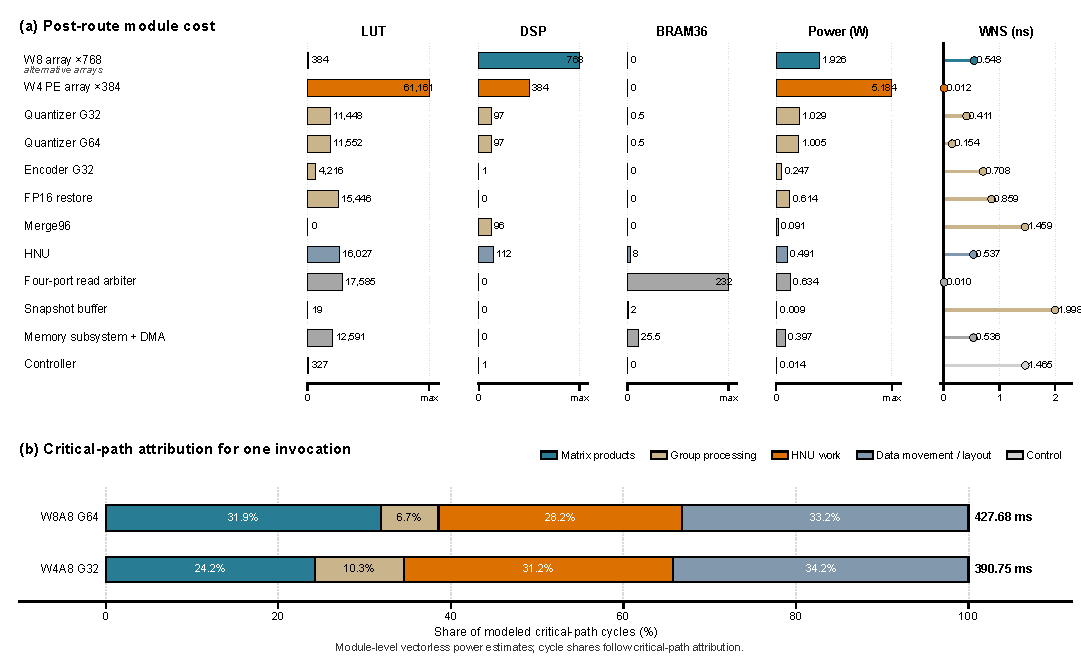
\includegraphics[width=.98\textwidth]{figures/fig12_impl_breakdown.pdf}
\caption{Module implementation costs and execution-time distribution. (a) Resource and power columns are independently scaled and labeled with their values; WNS is relative to zero slack. (b) Critical-path time is grouped by hardware responsibility.}\label{fig:impl_breakdown}
\end{figure*}

The W8A8 G64 results in Fig.~\ref{fig:impl_breakdown} connect implementation costs to execution time. Matrix products account for 31.9\% of critical-path cycles and group processing accounts for 6.7\%. HNU work, including nonlinear, reduction, and elementwise operations, accounts for 28.2\%; data movement and layout account for 33.2\%. The complete invocation takes 427.68 ms.

\subsection{Operating-point interpretation}
W8A8 G64 is the selected hardware operating point. Its numerical reference matches the floating-point selection-set total, while G64 produces fewer reduction groups than G32. The resource and schedule results show that scale handling, nonlinear work, and data movement must be considered together with packed multiplication when implementing this configuration.

\section{Related Work and Discussion}\label{sec:related}
\subsection{Comparison with FPGA accelerators}
Table~\ref{tab:sota_comparison} compares FPGA accelerators for vision transformers, language models, and robot action planning. The reported configurations span INT8 vision processing, mixed-precision language inference, and INT8 action generation. Vela targets the complete TurboVLA policy invocation, including visual processing, cross-modal interaction, and action prediction.

\begin{table*}[t]\centering\scriptsize
\setlength{\tabcolsep}{3pt}
\caption{Comparison with FPGA-based Transformer and embodied-AI accelerators.}\label{tab:sota_comparison}
\resizebox{\textwidth}{!}{%
\begin{tabular}{lcccccc}\toprule
Metric & \shortstack{TCAS-I'23\\\cite{huang2023integer}} & \shortstack{TCAS-I'25\\\cite{dong2025window}} & \shortstack{TCAS-I'25\\\cite{huang2025edgellm}} & \shortstack{HPCA'23\\\cite{dong2023heatvit}} & \shortstack{A-SSCC'25\\\cite{ma2025planner}} & \textbf{This Work}\\\midrule
FPGA & XCZU9EG & XCU50 & XCVU37P & XCZU9EG & XCZU7EV & XCZU7EV\\
Application & General CV & General CV & Language modeling & General CV & Robot control & End-to-end VLA\\
Model & ViT-S, ViT-B & Swin-Transformer & Qwen-7B & DeiT-S & $\pi_0$ action expert & TurboVLA\\
Precision & INT8 & INT8 & FP16/INT4 & INT8 & INT8 & W8A8 (G64)\\
Frequency (MHz) & 300 & 170 & 140 & 300 & 200 & 300\\
kLUTs / DSPs & 144 / 1,268 & 472.3 / 2,164 & 1,303 / 9,024 & 145 / 1,955 & 76.5 / 1,599 & $78.147 / 1,075^{a}$\\
Power (W) & 29.6 & 18.4 & 56.8 & 10.697 & 8.02 & $6.03^{a}$\\
Throughput (GOPS) & 762.7 & 830.26 & 1,260 & 220.6 & 903.2 & $921.6^{b}$\\
Throughput / power (GOPS/W) & 25.77 & 45.12 & 22.26 & 20.62 & 112.69 & $152.84^{a,b}$\\\bottomrule
\end{tabular}}
\par\vspace{3pt}\begin{minipage}{\textwidth}\scriptsize
Prior-work figures follow the comparison reported by Ma \emph{et al.}~\cite{ma2025planner}, Fig. 6.
$^{a}$This-work resources and power are module-subtotal estimates: the Table~\ref{tab:impl} W8 configuration with one G64 quantizer and one G32 encoder, plus one 0.60 W static-power contribution. Downstream group accumulators are outside the reported multiplier hierarchy. The 1,075 DSP subtotal includes the 977-DSP ablation budget and 98 quantizer/encoder DSPs.
$^{b}$Theoretical matrix peak with two operations per MAC; 152.84 is the ratio of that peak to the 6.03 W module-based estimate.
\end{minipage}
\end{table*}

The Pack2 array contains 768 matrix DSPs and generates two products per DSP cycle. Counting a multiplication and accumulation as two operations gives
\begin{equation}
P_{\mathrm{peak}}=768\times2\times2\times0.300=921.6\ \mathrm{GOPS}.
\end{equation}
Combining this peak with the 6.03 W module-based estimate yields 152.84 GOPS/W. The end-to-end evaluation separately reports 427.68 ms per TurboVLA invocation, covering matrix, group-processing, nonlinear, and data-movement work.

Huang \emph{et al.}~\cite{huang2023integer} combine integer-only execution with a group-vector systolic organization for vision transformers. Dong \emph{et al.}~\cite{dong2025window} exploit mixed-granularity sparsity in window-based transformers, while HeatViT~\cite{dong2023heatvit} dynamically selects image tokens and reuses backbone hardware for token selection. Vela focuses on a different source of cost: independently scaled reduction groups in a closed-loop VLA policy. Its quantization granularity is selected using robot-task success rates, and its arithmetic datapath explicitly handles group-result snapshots and scale-aligned merging.

EdgeLLM~\cite{huang2025edgellm} combines CPU--FPGA execution with mixed-precision operators, group-vector arrays, and overlapped data transfer for large language models. Vela uses W8A8 for both static-weight matrix products and dynamic attention, with an FP16-facing HNU for the heterogeneous operators in TurboVLA. This organization couples packed matrix execution to group quantization, result restoration, and shared nonlinear arithmetic.

The A-SSCC'25 accelerator~\cite{ma2025planner} is the closest application-level comparison and uses the same XCZU7EV device. It accelerates the $\pi_0$ action expert through behavior prediction and hierarchical tile-aware layer fusion, while vision--language semantic processing supplies its KV inputs. Vela instead spans the end-to-end TurboVLA invocation. The two designs address complementary costs: temporal prediction and fusion reduce action-planning work, whereas grouped quantization, Pack2, and HNU sharing reduce the execution cost of Vela's multimodal workload.

\subsection{Quantization methods}
SmoothQuant transfers activation quantization difficulty to weights through an equivalent channel transformation, enabling W8A8 post-training quantization in language models~\cite{smoothquant}. AWQ uses calibration activations to identify salient weight channels and selects scaling factors for low-bit, weight-only inference~\cite{awq}. The present work compares closed-loop W8A8 and W4A8 quality under the same selected robot tasks and implements a W8A8 G64 architecture. Its hardware concern is the runtime production of $K$-group activation scales and the merge of differently scaled integer partial sums. AWQ's weight-only W4A16 setting uses a different activation precision from this architecture. The Direct result in Section~\ref{sec:observations} isolates grouping granularity within this paper's numerical reference.

\subsection{VLA inference acceleration}
EfficientVLA combines language-layer pruning, task-aware visual-token selection, and feature caching in the diffusion action head~\cite{yang2025efficientvla}. SP-VLA jointly schedules a full VLA and a lightweight action generator, then prunes visual tokens using spatial and semantic importance~\cite{li2026spvla}. Action-aware Dynamic Pruning uses instruction relevance to select tokens and recent action trajectories to control pruning across manipulation stages~\cite{pei2026adp}. These methods reduce the frequency or size of inference work. Vela accelerates the retained operators through grouped quantization, scale-aligned merging, and packed arithmetic.

Asynchronous execution addresses the interaction between inference and robot motion. VLASH predicts the robot state at the future execution time from the preceding action chunk, aligning new predictions with continued action execution~\cite{tang2025vlash}. Its focus is reaction latency and prediction--execution alignment. Vela's cycle-level evaluation measures the hardware service time of one policy invocation; H1--H3 reduce the cost of the computation that an execution scheduler requests.

\subsection{Embodied action and VLA processors}
Algorithm--hardware co-design for robotic computing spans sensing, decision-making, and control~\cite{yan2025robotic_computing}. DADU-Corki predicts near-future trajectories to reduce model-invocation frequency, accelerates their conversion to torque commands, and overlaps communication with computation~\cite{huang2025daducorki}. This changes how often the policy runs and how its output reaches the robot. Vela instead organizes the arithmetic within each invocation, from group quantization to matrix products and nonlinear processing.

Zhang \emph{et al.} present a dedicated diffusion-based robot-manipulation SoC combining speculation and disturbance enhancement, with 94-Hz inference and 7.4-mJ/epoch fine-tuning~\cite{zhang2025robot_soc}. Ma \emph{et al.} map behavior prediction and tiled layer fusion to an FPGA action-planning accelerator~\cite{ma2025planner}. Wang \emph{et al.} span the vision--language model and action expert using SimHash-based token filtering and hybrid RRAM--SRAM processing near memory~\cite{wang2026vlaedge}. Together, these designs exploit temporal structure, specialized silicon, and data locality. Vela's FPGA contribution is the coordinated W8A8 datapath for group scales, packed products, and heterogeneous nonlinear operators.

DiTPA identifies action-, denoising-, and modality-level redundancy in a DiT action planner. It maps action prediction, alternating denoising with feature reuse, and calibrated multimodal skipping to dedicated hardware~\cite{ditpa}. Vela focuses on the execution of the complete TurboVLA invocation: H1 coordinates independently scaled products, H2 packs INT8 arithmetic, and H3 serves nonlinear and reduction operators. These mechanisms accelerate retained computation and complement approaches that reduce repeated action-planning work.

\subsection{Diffusion transformer reuse}
RADiT checks blockwise similarity across diffusion timesteps and reuses the preceding result when its dynamic threshold permits~\cite{park2025radit}. DSTAR combines fine-grained quantization of differential activations in linear layers with sparse attention reuse~\cite{zhang2026dstar}. Kaleido exploits channel-wise spatial and temporal correlations in video diffusion latents, using partial-result reuse and hardware data dispatch to serve the resulting irregular work~\cite{miao2026kaleido}. All three reduce repeated DiT computation. Their opportunities depend on timestep or latent correlations; this paper characterizes a specific VLA invocation and its quantization groups without assuming that such reuse is available in the traced workload. In particular, DSTAR's low-bit differential activation is a different numerical object from the complete group activations quantized by H1.

\subsection{Matrix arrays and heterogeneous operators}
DiP changes the input schedule and weight-stationary dataflow of a systolic array to remove synchronization FIFOs~\cite{abdelmaksoud2026dip}. Transitive Array instead constructs a result-reuse graph for binary GEMM and schedules dependent reuse across lanes~\cite{guo2025transitive}. DSP-Packing studies how wide FPGA multipliers can perform multiple narrow products and how packing errors are corrected~\cite{dsppacking}. H2 uses the DSP pre-adder to remove offset terms before multiplication, then sends recovered signed products to group accumulators. H1 supplies scale-aligned merging downstream. The HNU adds shared elementwise PWL arithmetic, row reductions, and an asymmetric set of special-function units for operators outside GEMM. These components target costs that product density, array input scheduling, and result reuse alone do not quantify in this VLA trace.

\section{Conclusion}
Grouped W8A8 VLA execution couples task quality to scale processing, arithmetic mapping, and heterogeneous operator service. The proposed FPGA architecture addresses these costs through H1 group quantization and merging, H2 Pack2 DSP products, and H3 nonlinear and reduction paths. The W8A8 G64 numerical reference achieves 153/160 successes, matching the floating-point aggregate, while the cycle model gives 427.68 ms per invocation at 300 MHz. The study shows why packed multiplication must be evaluated together with result handling and nonlinear work. Post-route module results quantify the implementation costs of these components.

\bibliographystyle{IEEEtran}
\bibliography{references,references_added}
\end{document}
